\documentclass[
  doc,
  floatsintext,
  longtable,
  a4paper,
  nolmodern,
  notxfonts,
  notimes,
  12pt,
  colorlinks=true,linkcolor=blue,citecolor=blue,urlcolor=blue]{apa7}

\usepackage{amsmath}
\usepackage{amssymb}

\geometry{inner=1in, outer=1in}
\fancyhfoffset[LE,RO]{0cm}


\usepackage[bidi=default]{babel}
\babelprovide[main,import]{spanish}


% get rid of language-specific shorthands (see #6817):
\let\LanguageShortHands\languageshorthands
\def\languageshorthands#1{}

\RequirePackage{longtable}
\RequirePackage{threeparttablex}

\makeatletter
\renewcommand{\paragraph}{\@startsection{paragraph}{4}{\parindent}%
	{0\baselineskip \@plus 0.2ex \@minus 0.2ex}%
	{-.5em}%
	{\normalfont\normalsize\bfseries\typesectitle}}

\renewcommand{\subparagraph}[1]{\@startsection{subparagraph}{5}{0.5em}%
	{0\baselineskip \@plus 0.2ex \@minus 0.2ex}%
	{-\z@\relax}%
	{\normalfont\normalsize\bfseries\itshape\hspace{\parindent}{#1}\textit{\addperi}}{\relax}}
\makeatother




\usepackage{longtable, booktabs, multirow, multicol, colortbl, hhline, caption, array, float, xpatch}
\usepackage{subcaption}


\renewcommand\thesubfigure{\Alph{subfigure}}
\setcounter{topnumber}{2}
\setcounter{bottomnumber}{2}
\setcounter{totalnumber}{4}
\renewcommand{\topfraction}{0.85}
\renewcommand{\bottomfraction}{0.85}
\renewcommand{\textfraction}{0.15}
\renewcommand{\floatpagefraction}{0.7}

\usepackage{tcolorbox}
\tcbuselibrary{listings,theorems, breakable, skins}
\usepackage{fontawesome5}

\definecolor{quarto-callout-color}{HTML}{909090}
\definecolor{quarto-callout-note-color}{HTML}{0758E5}
\definecolor{quarto-callout-important-color}{HTML}{CC1914}
\definecolor{quarto-callout-warning-color}{HTML}{EB9113}
\definecolor{quarto-callout-tip-color}{HTML}{00A047}
\definecolor{quarto-callout-caution-color}{HTML}{FC5300}
\definecolor{quarto-callout-color-frame}{HTML}{ACACAC}
\definecolor{quarto-callout-note-color-frame}{HTML}{4582EC}
\definecolor{quarto-callout-important-color-frame}{HTML}{D9534F}
\definecolor{quarto-callout-warning-color-frame}{HTML}{F0AD4E}
\definecolor{quarto-callout-tip-color-frame}{HTML}{02B875}
\definecolor{quarto-callout-caution-color-frame}{HTML}{FD7E14}

%\newlength\Oldarrayrulewidth
%\newlength\Oldtabcolsep


\usepackage{hyperref}



\usepackage{color}
\usepackage{fancyvrb}
\newcommand{\VerbBar}{|}
\newcommand{\VERB}{\Verb[commandchars=\\\{\}]}
\DefineVerbatimEnvironment{Highlighting}{Verbatim}{commandchars=\\\{\}}
% Add ',fontsize=\small' for more characters per line
\usepackage{framed}
\definecolor{shadecolor}{RGB}{241,243,245}
\newenvironment{Shaded}{\begin{snugshade}}{\end{snugshade}}
\newcommand{\AlertTok}[1]{\textcolor[rgb]{0.68,0.00,0.00}{#1}}
\newcommand{\AnnotationTok}[1]{\textcolor[rgb]{0.37,0.37,0.37}{#1}}
\newcommand{\AttributeTok}[1]{\textcolor[rgb]{0.40,0.45,0.13}{#1}}
\newcommand{\BaseNTok}[1]{\textcolor[rgb]{0.68,0.00,0.00}{#1}}
\newcommand{\BuiltInTok}[1]{\textcolor[rgb]{0.00,0.23,0.31}{#1}}
\newcommand{\CharTok}[1]{\textcolor[rgb]{0.13,0.47,0.30}{#1}}
\newcommand{\CommentTok}[1]{\textcolor[rgb]{0.37,0.37,0.37}{#1}}
\newcommand{\CommentVarTok}[1]{\textcolor[rgb]{0.37,0.37,0.37}{\textit{#1}}}
\newcommand{\ConstantTok}[1]{\textcolor[rgb]{0.56,0.35,0.01}{#1}}
\newcommand{\ControlFlowTok}[1]{\textcolor[rgb]{0.00,0.23,0.31}{\textbf{#1}}}
\newcommand{\DataTypeTok}[1]{\textcolor[rgb]{0.68,0.00,0.00}{#1}}
\newcommand{\DecValTok}[1]{\textcolor[rgb]{0.68,0.00,0.00}{#1}}
\newcommand{\DocumentationTok}[1]{\textcolor[rgb]{0.37,0.37,0.37}{\textit{#1}}}
\newcommand{\ErrorTok}[1]{\textcolor[rgb]{0.68,0.00,0.00}{#1}}
\newcommand{\ExtensionTok}[1]{\textcolor[rgb]{0.00,0.23,0.31}{#1}}
\newcommand{\FloatTok}[1]{\textcolor[rgb]{0.68,0.00,0.00}{#1}}
\newcommand{\FunctionTok}[1]{\textcolor[rgb]{0.28,0.35,0.67}{#1}}
\newcommand{\ImportTok}[1]{\textcolor[rgb]{0.00,0.46,0.62}{#1}}
\newcommand{\InformationTok}[1]{\textcolor[rgb]{0.37,0.37,0.37}{#1}}
\newcommand{\KeywordTok}[1]{\textcolor[rgb]{0.00,0.23,0.31}{\textbf{#1}}}
\newcommand{\NormalTok}[1]{\textcolor[rgb]{0.00,0.23,0.31}{#1}}
\newcommand{\OperatorTok}[1]{\textcolor[rgb]{0.37,0.37,0.37}{#1}}
\newcommand{\OtherTok}[1]{\textcolor[rgb]{0.00,0.23,0.31}{#1}}
\newcommand{\PreprocessorTok}[1]{\textcolor[rgb]{0.68,0.00,0.00}{#1}}
\newcommand{\RegionMarkerTok}[1]{\textcolor[rgb]{0.00,0.23,0.31}{#1}}
\newcommand{\SpecialCharTok}[1]{\textcolor[rgb]{0.37,0.37,0.37}{#1}}
\newcommand{\SpecialStringTok}[1]{\textcolor[rgb]{0.13,0.47,0.30}{#1}}
\newcommand{\StringTok}[1]{\textcolor[rgb]{0.13,0.47,0.30}{#1}}
\newcommand{\VariableTok}[1]{\textcolor[rgb]{0.07,0.07,0.07}{#1}}
\newcommand{\VerbatimStringTok}[1]{\textcolor[rgb]{0.13,0.47,0.30}{#1}}
\newcommand{\WarningTok}[1]{\textcolor[rgb]{0.37,0.37,0.37}{\textit{#1}}}

\providecommand{\tightlist}{%
  \setlength{\itemsep}{0pt}\setlength{\parskip}{0pt}}
\usepackage{longtable,booktabs,array}
\newcounter{none} % for unnumbered tables
\usepackage{calc} % for calculating minipage widths
% Correct order of tables after \paragraph or \subparagraph
\usepackage{etoolbox}
\makeatletter
\patchcmd\longtable{\par}{\if@noskipsec\mbox{}\fi\par}{}{}
\makeatother
% Allow footnotes in longtable head/foot
\IfFileExists{footnotehyper.sty}{\usepackage{footnotehyper}}{\usepackage{footnote}}
\makesavenoteenv{longtable}

\usepackage{graphicx}
\makeatletter
\newsavebox\pandoc@box
\newcommand*\pandocbounded[1]{% scales image to fit in text height/width
  \sbox\pandoc@box{#1}%
  \Gscale@div\@tempa{\textheight}{\dimexpr\ht\pandoc@box+\dp\pandoc@box\relax}%
  \Gscale@div\@tempb{\linewidth}{\wd\pandoc@box}%
  \ifdim\@tempb\p@<\@tempa\p@\let\@tempa\@tempb\fi% select the smaller of both
  \ifdim\@tempa\p@<\p@\scalebox{\@tempa}{\usebox\pandoc@box}%
  \else\usebox{\pandoc@box}%
  \fi%
}
% Set default figure placement to htbp
\def\fps@figure{htbp}
\makeatother







\usepackage{newtx}

\defaultfontfeatures{Scale=MatchLowercase}
\defaultfontfeatures[\rmfamily]{Ligatures=TeX,Scale=1}





\title{Guía Completa de Ranger}


\shorttitle{Guía Completa de Ranger}


\usepackage{etoolbox}



\ccoppy{\textcopyright~2025}



\author{Edison Achalma}



\affiliation{
{Escuela Profesional de Economía, Universidad Nacional de San Cristóbal
de Huamanga}}




\leftheader{Achalma}

\date{2025-12-30}


\abstract{Ranger es un gestor de archivos basado en consola altamente
eficiente, diseñado con una fuerte inspiración en los atajos de teclado
de Vim y una filosofía minimalista. Esta guía completa explora en
detalle su instalación en diferentes sistemas operativos, configuración
inicial y avanzada, estructura de archivos de configuración (rc.conf,
rifle.conf, scope.sh, commands.py), así como la personalización profunda
mediante mapeos de teclado, comandos personalizados en Python y plugins.
Se detallan las características principales que lo distinguen;
navegación multi-columna, previsualización automática de múltiples tipos
de archivo (texto, código, imágenes, PDFs, videos, comprimidos), gestión
inteligente de archivos mediante rifle, soporte de pestañas, marcadores,
renombrado masivo, integración con el shell y capacidades de preview
mejoradas mediante herramientas externas. La guía incluye referencias
prácticas de atajos fundamentales y avanzados, ejemplos de configuración
realistas, soluciones a problemas comunes, trucos de productividad y
recomendaciones para integrar Ranger en flujos de trabajo diarios de
usuarios de terminal (especialmente aquellos familiarizados con
Vim/Neovim). Dirigida tanto a usuarios noveles que buscan reemplazar
gestores gráficos tradicionales, como a usuarios avanzados que desean
optimizar y extender al máximo esta poderosa herramienta de gestión de
archivos en entornos Linux. }

\keywords{Vim, Ranger, File Manager}

\authornote{\par{\addORCIDlink{Edison Achalma}{0000-0001-6996-3364}} 
\par{ }
\par{   El autor no tiene conflictos de interés que revelar.    Los
roles de autor se clasificaron utilizando la taxonomía de roles de
colaborador (CRediT; https://credit.niso.org/) de la siguiente
manera:  Edison Achalma:   conceptualización, metodología, análisis
formal, investigación, recursos, curación de
datos, redacción, visualización, supervisión, administración del
proyecto}
\par{La correspondencia relativa a este artículo debe dirigirse a Edison
Achalma, Escuela Profesional de Economía, Universidad Nacional de San
Cristóbal de Huamanga, Portal Independencia N°
57, Ayacucho, AYA 5001, Perú, Email: \href{mailto:elmer.achalma.09@unsch.edu.pe}{elmer.achalma.09@unsch.edu.pe}}
}

\makeatletter
\let\endoldlt\endlongtable
\def\endlongtable{
\hline
\endoldlt
}
\makeatother

\urlstyle{same}



\hypersetup{
  pdftitle={Gu\'{\i}a Completa de Ranger},
  pdfauthor={Autor}
}
\makeatletter
\@ifpackageloaded{caption}{}{\usepackage{caption}}
\AtBeginDocument{%
\ifdefined\contentsname
  \renewcommand*\contentsname{Tabla de contenidos}
\else
  \newcommand\contentsname{Tabla de contenidos}
\fi
\ifdefined\listfigurename
  \renewcommand*\listfigurename{Lista de Figuras}
\else
  \newcommand\listfigurename{Lista de Figuras}
\fi
\ifdefined\listtablename
  \renewcommand*\listtablename{Lista de Tablas}
\else
  \newcommand\listtablename{Lista de Tablas}
\fi
\ifdefined\figurename
  \renewcommand*\figurename{Figura}
\else
  \newcommand\figurename{Figura}
\fi
\ifdefined\tablename
  \renewcommand*\tablename{Tabla}
\else
  \newcommand\tablename{Tabla}
\fi
}
\@ifpackageloaded{float}{}{\usepackage{float}}
\floatstyle{ruled}
\@ifundefined{c@chapter}{\newfloat{codelisting}{h}{lop}}{\newfloat{codelisting}{h}{lop}[chapter]}
\floatname{codelisting}{Listado}
\newcommand*\listoflistings{\listof{codelisting}{Lista de Listados}}
\makeatother
\makeatletter
\makeatother
\makeatletter
\@ifpackageloaded{caption}{}{\usepackage{caption}}
\@ifpackageloaded{subcaption}{}{\usepackage{subcaption}}
\makeatother
\makeatletter
\@ifpackageloaded{fontawesome5}{}{\usepackage{fontawesome5}}
\makeatother

% From https://tex.stackexchange.com/a/645996/211326
%%% apa7 doesn't want to add appendix section titles in the toc
%%% let's make it do it
\makeatletter
\xpatchcmd{\appendix}
  {\par}
  {\addcontentsline{toc}{section}{\@currentlabelname}\par}
  {}{}
\makeatother

%% Disable longtable counter
%% https://tex.stackexchange.com/a/248395/211326

\usepackage{etoolbox}

\makeatletter
\patchcmd{\LT@caption}
  {\bgroup}
  {\bgroup\global\LTpatch@captiontrue}
  {}{}
\patchcmd{\longtable}
  {\par}
  {\par\global\LTpatch@captionfalse}
  {}{}
\apptocmd{\endlongtable}
  {\ifLTpatch@caption\else\addtocounter{table}{-1}\fi}
  {}{}
\newif\ifLTpatch@caption
\makeatother

\begin{document}

\maketitle


\hypertarget{toc}{}
\tableofcontents
\newpage
\section[Introduction]{Guía Completa de Ranger}

\setcounter{secnumdepth}{3}

\setlength\LTleft{0pt}




\pandocbounded{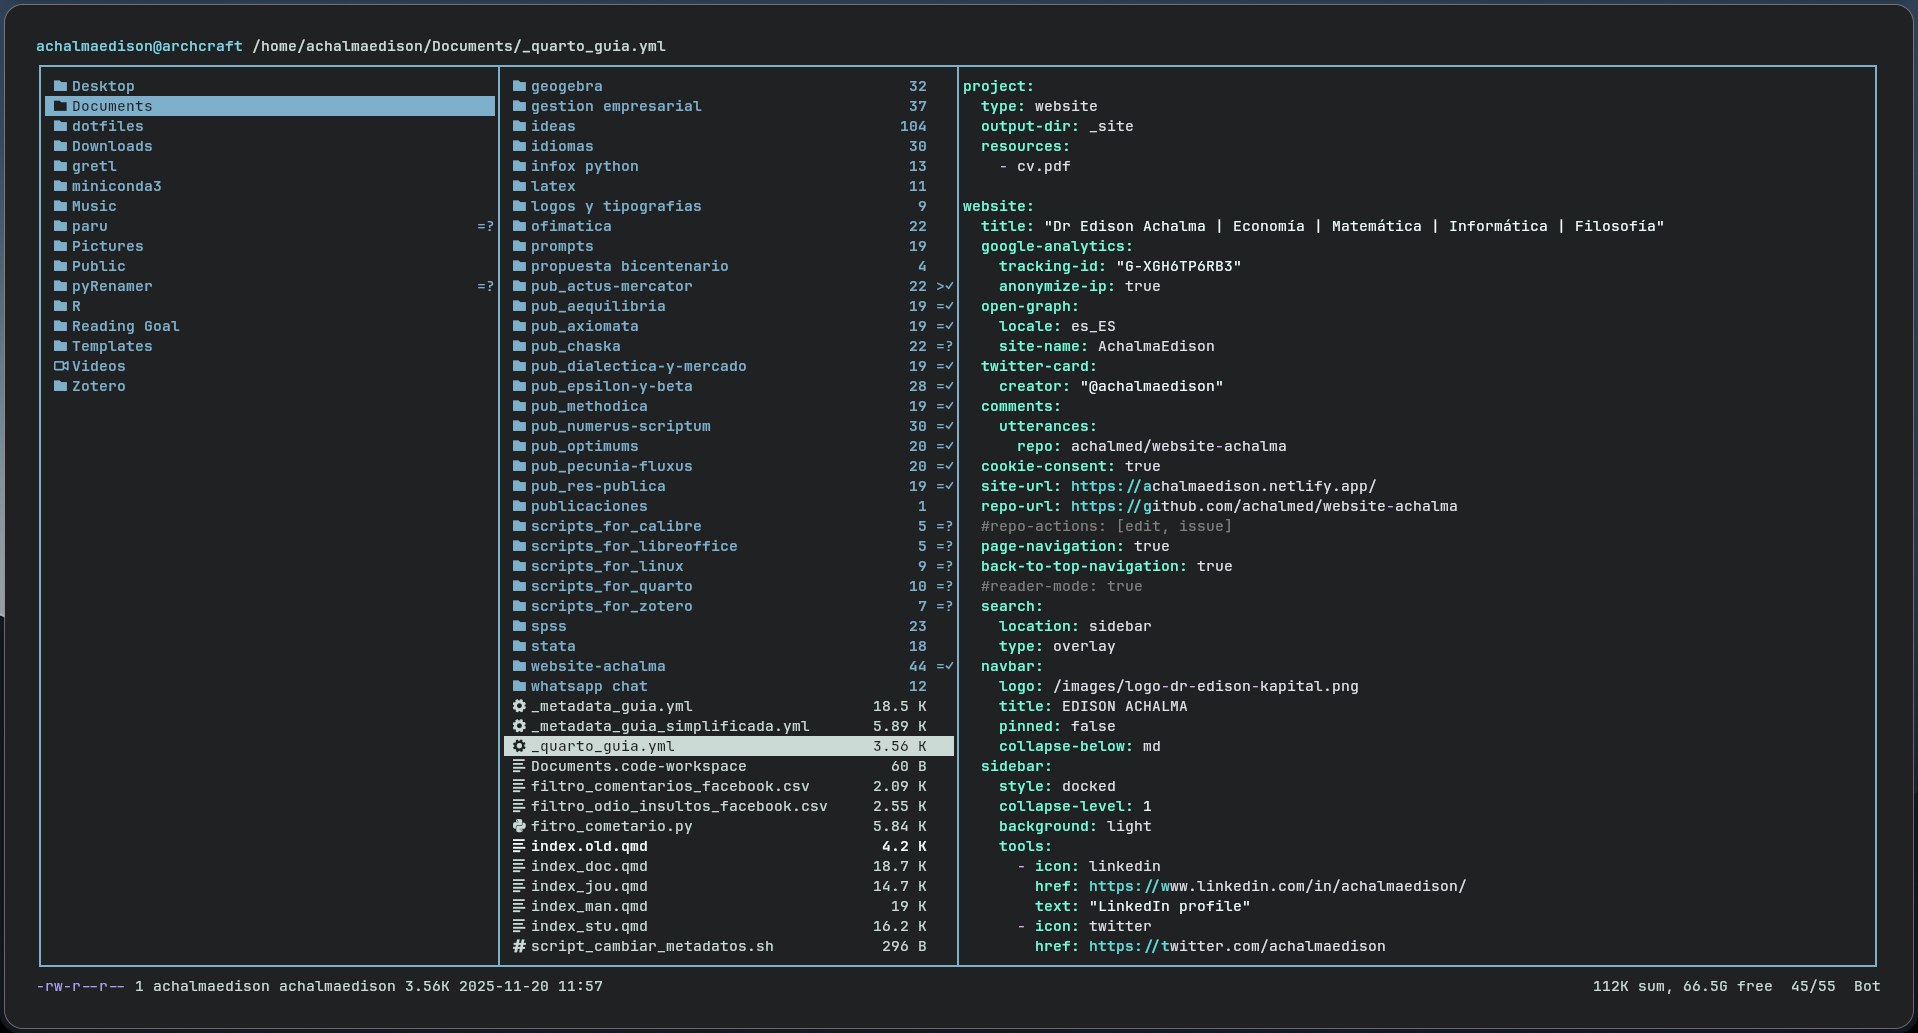
\includegraphics[keepaspectratio]{featured.png}}

\textbf{¿Qué es Ranger?}

Ranger es un gestor de archivos de consola con:

\begin{itemize}
\tightlist
\item
  Atajos de teclado inspirados en Vim
\item
  Interfaz minimalista con curses
\item
  Vista de jerarquía de directorios (multi-columna)
\item
  Previsualización automática de archivos
\item
  Integración con rifle (lanzador de archivos inteligente)
\end{itemize}

\textbf{Filosofía de Diseño}

\begin{itemize}
\tightlist
\item
  \textbf{Mantenible}: Escrito en Python de alto nivel
\item
  \textbf{Rápido}: Cambiar directorios y navegar eficientemente
\item
  \textbf{Minimalista}: Pequeño pero útil, hace una cosa bien
\item
  \textbf{Integrado}: Perfecta integración con el shell Unix
\end{itemize}

\textbf{Características Principales}

\begin{itemize}
\tightlist
\item
  Soporte UTF-8\\
\item
  Pantalla multi-columna\\
\item
  Previsualización del archivo/directorio seleccionado\\
\item
  Operaciones comunes con archivos (crear/chmod/copiar/eliminar)\\
\item
  Renombrado múltiple de archivos\\
\item
  Consola y atajos estilo VIM\\
\item
  Determina tipos de archivo automáticamente\\
\item
  Pestañas, marcadores, soporte de ratón\\
\item
  Cambia el directorio del shell al salir
\end{itemize}

\section{Instalación}\label{instalaciuxf3n}

\subsection{Desde Repositorios}\label{desde-repositorios}

\textbf{Ubuntu/Debian:}

\begin{Shaded}
\begin{Highlighting}[]
\FunctionTok{sudo}\NormalTok{ apt{-}get update}
\FunctionTok{sudo}\NormalTok{ apt{-}get install ranger}
\end{Highlighting}
\end{Shaded}

\textbf{Fedora:}

\begin{Shaded}
\begin{Highlighting}[]
\FunctionTok{sudo}\NormalTok{ dnf install ranger}
\end{Highlighting}
\end{Shaded}

\textbf{Arch Linux:}

\begin{Shaded}
\begin{Highlighting}[]
\FunctionTok{sudo}\NormalTok{ pacman }\AttributeTok{{-}S}\NormalTok{ ranger}
\end{Highlighting}
\end{Shaded}

\textbf{macOS (Homebrew):}

\begin{Shaded}
\begin{Highlighting}[]
\ExtensionTok{brew}\NormalTok{ install ranger}
\end{Highlighting}
\end{Shaded}

\subsection{Desde PyPI}\label{desde-pypi}

\begin{Shaded}
\begin{Highlighting}[]
\ExtensionTok{pip}\NormalTok{ install ranger{-}fm}
\CommentTok{\# O mejor con pipx (entorno aislado)}
\ExtensionTok{pipx}\NormalTok{ install ranger{-}fm}
\end{Highlighting}
\end{Shaded}

\subsection{Desde Código Fuente}\label{desde-cuxf3digo-fuente}

\begin{Shaded}
\begin{Highlighting}[]
\FunctionTok{git}\NormalTok{ clone https://github.com/ranger/ranger.git}
\BuiltInTok{cd}\NormalTok{ ranger}
\FunctionTok{sudo}\NormalTok{ make install}
\end{Highlighting}
\end{Shaded}

\subsection{Verificar Instalación}\label{verificar-instalaciuxf3n}

\begin{Shaded}
\begin{Highlighting}[]
\ExtensionTok{ranger} \AttributeTok{{-}{-}version}
\end{Highlighting}
\end{Shaded}

\subsection{Dependencias Opcionales}\label{dependencias-opcionales}

Para habilitar todas las funcionalidades de previsualización y análisis
de archivos en \texttt{ranger}, se recomienda instalar las siguientes
dependencias según tu distribución.

\subsubsection{Para Debian / Ubuntu /
derivados}\label{para-debian-ubuntu-derivados}

\begin{Shaded}
\begin{Highlighting}[]
\CommentTok{\# Básico (casi imprescindible)}
\FunctionTok{sudo}\NormalTok{ apt install file}

\CommentTok{\# Resaltado de sintaxis (elige uno o varios)}
\FunctionTok{sudo}\NormalTok{ apt install highlight}
\FunctionTok{sudo}\NormalTok{ apt install bat}
\CommentTok{\# pygments vía pip si prefieres la versión python:}
\CommentTok{\# pip install {-}{-}user pygments}

\CommentTok{\# Imágenes (elige según tu terminal)}
\FunctionTok{sudo}\NormalTok{ apt install w3m w3m{-}img           }\CommentTok{\# Método clásico}
\FunctionTok{sudo}\NormalTok{ apt install caca{-}utils            }\CommentTok{\# Arte ASCII alternativo}
\CommentTok{\# kitty / wezterm / alacritty → mejor con ueberzugpp}

\CommentTok{\# Conversión y procesamiento de imágenes}
\FunctionTok{sudo}\NormalTok{ apt install imagemagick}

\CommentTok{\# Archivos comprimidos}
\FunctionTok{sudo}\NormalTok{ apt install atool unrar p7zip{-}full}

\CommentTok{\# PDFs}
\FunctionTok{sudo}\NormalTok{ apt install poppler{-}utils}

\CommentTok{\# Miniaturas de video}
\FunctionTok{sudo}\NormalTok{ apt install ffmpegthumbnailer}

\CommentTok{\# Información de medios}
\FunctionTok{sudo}\NormalTok{ apt install mediainfo}

\CommentTok{\# Idiomas y codificación especial}
\FunctionTok{sudo}\NormalTok{ apt install python3{-}chardet}
\ExtensionTok{pip}\NormalTok{ install }\AttributeTok{{-}{-}user}\NormalTok{ python{-}bidi        }\CommentTok{\# Para árabe, hebreo, etc.}

\CommentTok{\# Convertir SVG}
\FunctionTok{sudo}\NormalTok{ apt{-}get install librsvg2{-}bin}
\end{Highlighting}
\end{Shaded}

\subsubsection{Para Arch Linux / Manjaro /
derivados}\label{para-arch-linux-manjaro-derivados}

\begin{Shaded}
\begin{Highlighting}[]
\CommentTok{\# Básico (casi imprescindible)}
\FunctionTok{sudo}\NormalTok{ pacman }\AttributeTok{{-}S}\NormalTok{ file}

\CommentTok{\# Resaltado de sintaxis (elige uno o varios)}
\FunctionTok{sudo}\NormalTok{ pacman }\AttributeTok{{-}S}\NormalTok{ highlight}
\FunctionTok{sudo}\NormalTok{ pacman }\AttributeTok{{-}S}\NormalTok{ bat}
\CommentTok{\# pygments vía pip si prefieres:}
\CommentTok{\# pip install {-}{-}user pygments}

\CommentTok{\# Imágenes (elige según tu terminal)}
\FunctionTok{sudo}\NormalTok{ pacman }\AttributeTok{{-}S}\NormalTok{ w3m libcaca             }\CommentTok{\# Método clásico + ASCII}
\FunctionTok{sudo}\NormalTok{ pacman }\AttributeTok{{-}S}\NormalTok{ ueberzugpp              }\CommentTok{\# Muy recomendado (mejor que w3m)}
\CommentTok{\# kitty / wezterm → soporte nativo excelente}

\CommentTok{\# Conversión y procesamiento de imágenes}
\FunctionTok{sudo}\NormalTok{ pacman }\AttributeTok{{-}S}\NormalTok{ imagemagick}

\CommentTok{\# Archivos comprimidos}
\FunctionTok{sudo}\NormalTok{ pacman }\AttributeTok{{-}S}\NormalTok{ atool unrar p7zip}

\CommentTok{\# PDFs}
\FunctionTok{sudo}\NormalTok{ pacman }\AttributeTok{{-}S}\NormalTok{ poppler}

\CommentTok{\# Miniaturas de video}
\FunctionTok{sudo}\NormalTok{ pacman }\AttributeTok{{-}S}\NormalTok{ ffmpegthumbnailer}

\CommentTok{\# Información de medios}
\FunctionTok{sudo}\NormalTok{ pacman }\AttributeTok{{-}S}\NormalTok{ mediainfo}

\CommentTok{\# Idiomas y codificación especial}
\FunctionTok{sudo}\NormalTok{ pacman }\AttributeTok{{-}S}\NormalTok{ python{-}chardet}
\FunctionTok{sudo}\NormalTok{ pacman }\AttributeTok{{-}S}\NormalTok{ python{-}bidi             }\CommentTok{\# Para textos RTL (árabe, hebreo...)}

\CommentTok{\# Convertir SVG}
\FunctionTok{sudo}\NormalTok{ pacman }\AttributeTok{{-}S}\NormalTok{ librsvg}
\end{Highlighting}
\end{Shaded}

\subsubsection{Instalación recomendada mínima (elige según tu
caso)}\label{instalaciuxf3n-recomendada-muxednima-elige-seguxfan-tu-caso}

\textbf{Usuario de Arch + kitty/wezterm:}

\begin{Shaded}
\begin{Highlighting}[]
\FunctionTok{sudo}\NormalTok{ pacman }\AttributeTok{{-}S}\NormalTok{ file highlight bat imagemagick ffmpegthumbnailer }\DataTypeTok{\textbackslash{}}
\NormalTok{poppler mediainfo ueberzugpp}
\CommentTok{\# Opcional pero muy útil:}
\FunctionTok{sudo}\NormalTok{ pacman }\AttributeTok{{-}S}\NormalTok{ atool unrar p7zip python{-}bidi python{-}chardet}
\end{Highlighting}
\end{Shaded}

\textbf{Usuario de Ubuntu + terminal clásico:}

\begin{Shaded}
\begin{Highlighting}[]
\FunctionTok{sudo}\NormalTok{ apt install file highlight imagemagick ffmpegthumbnailer }\DataTypeTok{\textbackslash{}}
\NormalTok{poppler{-}utils mediainfo w3m w3m{-}img atool unrar p7zip{-}full python3{-}chardet}
\CommentTok{\# Opcional: pip install {-}{-}user python{-}bidi}
\end{Highlighting}
\end{Shaded}

\section{Configuración Inicial}\label{configuraciuxf3n-inicial}

\subsection{Generar Archivos de
Configuración}\label{generar-archivos-de-configuraciuxf3n}

Ranger puede copiar automáticamente los archivos de configuración por
defecto:

\begin{Shaded}
\begin{Highlighting}[]
\CommentTok{\# Copiar todas las configuraciones}
\ExtensionTok{ranger} \AttributeTok{{-}{-}copy{-}config}\OperatorTok{=}\NormalTok{all}

\CommentTok{\# Copiar archivos específicos}
\ExtensionTok{ranger} \AttributeTok{{-}{-}copy{-}config}\OperatorTok{=}\NormalTok{rc          }\CommentTok{\# Configuración principal}
\ExtensionTok{ranger} \AttributeTok{{-}{-}copy{-}config}\OperatorTok{=}\NormalTok{rifle       }\CommentTok{\# Configuración de rifle}
\ExtensionTok{ranger} \AttributeTok{{-}{-}copy{-}config}\OperatorTok{=}\NormalTok{scope       }\CommentTok{\# Script de previsualización}
\ExtensionTok{ranger} \AttributeTok{{-}{-}copy{-}config}\OperatorTok{=}\NormalTok{commands    }\CommentTok{\# Comandos personalizados}
\end{Highlighting}
\end{Shaded}

\subsection{Ubicación de Archivos}\label{ubicaciuxf3n-de-archivos}

Los archivos de configuración se encuentran en:

\begin{Shaded}
\begin{Highlighting}[]
\ExtensionTok{\textasciitilde{}/.config/ranger/}
\ExtensionTok{├──}\NormalTok{ rc.conf           }\CommentTok{\# Configuración principal y atajos}
\ExtensionTok{├──}\NormalTok{ rifle.conf        }\CommentTok{\# Lanzador de archivos}
\ExtensionTok{├──}\NormalTok{ scope.sh          }\CommentTok{\# Script de previsualización}
\ExtensionTok{├──}\NormalTok{ commands.py       }\CommentTok{\# Comandos personalizados (Python)}
\ExtensionTok{├──}\NormalTok{ commands\_full.py  }\CommentTok{\# Comandos adicionales}
\ExtensionTok{└──}\NormalTok{ plugins/          }\CommentTok{\# Directorio para plugins}
\end{Highlighting}
\end{Shaded}

\subsection{Primer Lanzamiento}\label{primer-lanzamiento}

\begin{Shaded}
\begin{Highlighting}[]
\ExtensionTok{ranger}
\end{Highlighting}
\end{Shaded}

Al iniciar ranger por primera vez:

\begin{itemize}
\tightlist
\item
  Se abre en el directorio actual
\item
  Muestra tres columnas: padre, actual, previsualización
\item
  Usa las flechas o \texttt{hjkl} para navegar
\end{itemize}

\section{Interfaz y Navegación
Básica}\label{interfaz-y-navegaciuxf3n-buxe1sica}

\subsection{Estructura de la Pantalla}\label{estructura-de-la-pantalla}

\begin{Shaded}
\begin{Highlighting}[]
\ExtensionTok{┌─────────────────────────────────────────────────────────┐}
\ExtensionTok{│}\NormalTok{ Directorio Padre │ Directorio Actual │ Previsualización │}
\ExtensionTok{│}\NormalTok{                  │                   │                  │}
\ExtensionTok{│}\NormalTok{  parent/         │ }\OperatorTok{\textgreater{}}\NormalTok{ archivo1.txt    │ Contenido del    │}
\ExtensionTok{│}\NormalTok{  current/        │   archivo2.py     │ archivo1.txt...  │}
\ExtensionTok{│}\NormalTok{  sibling/        │   carpeta/        │                  │}
\ExtensionTok{│}\NormalTok{                  │   imagen.png      │                  │}
\ExtensionTok{│}\NormalTok{                  │                   │                  │}
\ExtensionTok{├─────────────────────────────────────────────────────────┤}
\ExtensionTok{│}\NormalTok{ Barra de Estado: PWD, permisos, tamaño, fecha           │}
\ExtensionTok{└─────────────────────────────────────────────────────────┘}
\end{Highlighting}
\end{Shaded}

\subsection{Columnas}\label{columnas}

\begin{enumerate}
\def\labelenumi{\arabic{enumi}.}
\tightlist
\item
  \textbf{Columna Izquierda}: Contenido del directorio padre
\item
  \textbf{Columna Central}: Directorio actual (principal)
\item
  \textbf{Columna Derecha}: Previsualización del archivo/directorio
  seleccionado
\end{enumerate}

\subsection{Barra de Estado}\label{barra-de-estado}

Muestra información del archivo seleccionado:

\begin{itemize}
\tightlist
\item
  Permisos (rwxr-xr-x)
\item
  Usuario y grupo propietario
\item
  Tamaño del archivo
\item
  Fecha de modificación
\item
  Ruta completa del directorio actual
\end{itemize}

\section{Atajos de Teclado
Fundamentales}\label{atajos-de-teclado-fundamentales}

\subsection{Navegación Básica (Estilo
Vim)}\label{navegaciuxf3n-buxe1sica-estilo-vim}

{\def\LTcaptype{none} % do not increment counter
\begin{longtable}[]{@{}ll@{}}
\toprule\noalign{}
Tecla & Acción \\
\midrule\noalign{}
\endhead
\bottomrule\noalign{}
\endlastfoot
\texttt{h} & Ir al directorio padre (arriba en jerarquía) \\
\texttt{j} & Mover cursor hacia abajo \\
\texttt{k} & Mover cursor hacia arriba \\
\texttt{l} & Entrar a directorio / Abrir archivo \\
\texttt{↑} & Mover cursor hacia arriba \\
\texttt{↓} & Mover cursor hacia abajo \\
\texttt{←} & Ir al directorio padre \\
\texttt{→} & Entrar a directorio / Abrir archivo \\
\end{longtable}
}

\subsection{Movimiento Rápido}\label{movimiento-ruxe1pido}

{\def\LTcaptype{none} % do not increment counter
\begin{longtable}[]{@{}ll@{}}
\toprule\noalign{}
Tecla & Acción \\
\midrule\noalign{}
\endhead
\bottomrule\noalign{}
\endlastfoot
\texttt{gg} & Ir al inicio de la lista \\
\texttt{G} & Ir al final de la lista \\
\texttt{H} & Ir al inicio de la pantalla visible \\
\texttt{M} & Ir a la mitad de la pantalla visible \\
\texttt{L} & Ir al final de la pantalla visible \\
\texttt{\{} & Subir una página \\
\texttt{\}} & Bajar una página \\
\texttt{Ctrl+u} & Media página arriba \\
\texttt{Ctrl+d} & Media página abajo \\
\texttt{Ctrl+b} & Página completa arriba \\
\texttt{Ctrl+f} & Página completa abajo \\
\end{longtable}
}

\subsection{Salir y Ayuda}\label{salir-y-ayuda}

{\def\LTcaptype{none} % do not increment counter
\begin{longtable}[]{@{}ll@{}}
\toprule\noalign{}
Tecla & Acción \\
\midrule\noalign{}
\endhead
\bottomrule\noalign{}
\endlastfoot
\texttt{q} & Salir de ranger \\
\texttt{Q} & Salir sin cambiar directorio \\
\texttt{?} & Abrir manual de ayuda \\
\texttt{W} & Ver log de ranger \\
\end{longtable}
}

\section{Navegación Avanzada}\label{navegaciuxf3n-avanzada}

\subsection{Historial de Navegación}\label{historial-de-navegaciuxf3n}

{\def\LTcaptype{none} % do not increment counter
\begin{longtable}[]{@{}ll@{}}
\toprule\noalign{}
Tecla & Acción \\
\midrule\noalign{}
\endhead
\bottomrule\noalign{}
\endlastfoot
\texttt{H} & Ir atrás en el historial (history back) \\
\texttt{L} & Ir adelante en el historial (history forward) \\
\texttt{Alt+Left} & Historial atrás \\
\texttt{Alt+Right} & Historial adelante \\
\end{longtable}
}

\subsection{Saltos Rápidos}\label{saltos-ruxe1pidos}

{\def\LTcaptype{none} % do not increment counter
\begin{longtable}[]{@{}ll@{}}
\toprule\noalign{}
Tecla & Acción \\
\midrule\noalign{}
\endhead
\bottomrule\noalign{}
\endlastfoot
\texttt{gh} & Ir a HOME \texttt{\textasciitilde{}} \\
\texttt{ge} & Ir a /etc \\
\texttt{gu} & Ir a /usr \\
\texttt{gd} & Ir a /dev \\
\texttt{go} & Ir a /opt \\
\texttt{gv} & Ir a /var \\
\texttt{gm} & Ir a /media \\
\texttt{gM} & Ir a /mnt \\
\texttt{gs} & Ir a /srv \\
\texttt{gR} & Ir a / (root) \\
\texttt{g/} & Ir a / (root) \\
\texttt{g?} & Ir a /usr/share/doc/ranger \\
\end{longtable}
}

\subsection{Navegación por Primera
Letra}\label{navegaciuxf3n-por-primera-letra}

{\def\LTcaptype{none} % do not increment counter
\begin{longtable}[]{@{}ll@{}}
\toprule\noalign{}
Tecla & Acción \\
\midrule\noalign{}
\endhead
\bottomrule\noalign{}
\endlastfoot
\texttt{f\textless{}letra\textgreater{}} & Buscar archivo que empiece
con letra \\
\texttt{F\textless{}letra\textgreater{}} & Buscar archivo que empiece
con letra (multi-match) \\
\end{longtable}
}

\textbf{Ejemplo:}

\begin{itemize}
\tightlist
\item
  \texttt{ft} - Salta al primer archivo que empiece con `t'
\item
  \texttt{Ft} - Salta a archivos que empiecen con `t', presiona
  \texttt{;} para siguiente
\end{itemize}

\subsection{Ir a Directorio
Específico}\label{ir-a-directorio-especuxedfico}

{\def\LTcaptype{none} % do not increment counter
\begin{longtable}[]{@{}ll@{}}
\toprule\noalign{}
Tecla & Acción \\
\midrule\noalign{}
\endhead
\bottomrule\noalign{}
\endlastfoot
\texttt{cd} & Abrir prompt para cambiar directorio \\
\texttt{:cd\ /ruta} & Ir a ruta específica \\
\texttt{:cd\ -} & Ir al directorio anterior \\
\end{longtable}
}

\section{Operaciones con Archivos}\label{operaciones-con-archivos}

\subsection{Copiar, Cortar y Pegar}\label{copiar-cortar-y-pegar}

{\def\LTcaptype{none} % do not increment counter
\begin{longtable}[]{@{}ll@{}}
\toprule\noalign{}
Tecla & Acción \\
\midrule\noalign{}
\endhead
\bottomrule\noalign{}
\endlastfoot
\texttt{yy} & Copiar (yank) archivo seleccionado \\
\texttt{dd} & Cortar (cut) archivo seleccionado \\
\texttt{pp} & Pegar archivo \\
\texttt{po} & Pegar sobrescribiendo \\
\texttt{pP} & Pegar creando enlaces simbólicos \\
\texttt{pO} & Pegar enlaces simbólicos sobrescribiendo \\
\texttt{pl} & Pegar creando enlaces duros (hardlinks) \\
\texttt{pL} & Pegar enlaces duros con nuevo nombre \\
\texttt{ud} & Deshacer (undo) operación de cortar \\
\texttt{uy} & Deshacer (undo) operación de copiar \\
\end{longtable}
}

\subsection{Eliminar}\label{eliminar}

{\def\LTcaptype{none} % do not increment counter
\begin{longtable}[]{@{}ll@{}}
\toprule\noalign{}
Tecla & Acción \\
\midrule\noalign{}
\endhead
\bottomrule\noalign{}
\endlastfoot
\texttt{dD} & Eliminar archivo (pide confirmación) \\
\texttt{dT} & Mover a papelera (si está configurada) \\
\end{longtable}
}

\subsection{Crear y Editar}\label{crear-y-editar}

{\def\LTcaptype{none} % do not increment counter
\begin{longtable}[]{@{}ll@{}}
\toprule\noalign{}
Tecla & Acción \\
\midrule\noalign{}
\endhead
\bottomrule\noalign{}
\endlastfoot
\texttt{:touch\ nombre} & Crear archivo nuevo \\
\texttt{:mkdir\ nombre} & Crear directorio nuevo \\
\texttt{i} & Mostrar nombre del archivo actual \\
\texttt{E} & Editar archivo con editor por defecto \\
\texttt{cw} & Renombrar archivo (change word) \\
\texttt{a} & Renombrar - cursor al final \\
\texttt{A} & Renombrar - cursor después de extensión \\
\texttt{I} & Renombrar - cursor al principio \\
\end{longtable}
}

\subsection{Permisos y Propiedades}\label{permisos-y-propiedades}

{\def\LTcaptype{none} % do not increment counter
\begin{longtable}[]{@{}ll@{}}
\toprule\noalign{}
Tecla & Acción \\
\midrule\noalign{}
\endhead
\bottomrule\noalign{}
\endlastfoot
\texttt{=} & Mostrar permisos en notación chmod \\
\texttt{+\textless{}permisos\textgreater{}} & Añadir permisos (ej:
\texttt{+x}) \\
\texttt{-\textless{}permisos\textgreater{}} & Quitar permisos (ej:
\texttt{-w}) \\
\end{longtable}
}

\textbf{Ejemplos:}

\begin{Shaded}
\begin{Highlighting}[]
\ExtensionTok{+x}    \CommentTok{\# Añadir permiso de ejecución}
\ExtensionTok{{-}w}    \CommentTok{\# Quitar permiso de escritura}
\ExtensionTok{=755}  \CommentTok{\# Establecer permisos exactos}
\end{Highlighting}
\end{Shaded}

\section{Selección Múltiple}\label{selecciuxf3n-muxfaltiple}

\subsection{Seleccionar Archivos}\label{seleccionar-archivos}

{\def\LTcaptype{none} % do not increment counter
\begin{longtable}[]{@{}ll@{}}
\toprule\noalign{}
Tecla & Acción \\
\midrule\noalign{}
\endhead
\bottomrule\noalign{}
\endlastfoot
\texttt{Space} & Marcar/desmarcar archivo y bajar \\
\texttt{v} & Invertir selección de todos los archivos \\
\texttt{V} & Entrar en modo visual (selección continua) \\
\texttt{uv} & Desmarcar todos los archivos \\
\end{longtable}
}

\subsection{Modo Visual}\label{modo-visual}

En modo visual (\texttt{V}):

\begin{itemize}
\tightlist
\item
  \texttt{j/k} - Extender selección arriba/abajo
\item
  \texttt{gg/G} - Seleccionar hasta inicio/final
\item
  \texttt{o} - Cambiar punto de anclaje de selección
\end{itemize}

\subsection{Operaciones con Múltiples
Archivos}\label{operaciones-con-muxfaltiples-archivos}

Una vez seleccionados:

\begin{itemize}
\tightlist
\item
  \texttt{yy} - Copiar todos los seleccionados
\item
  \texttt{dd} - Cortar todos los seleccionados
\item
  \texttt{dD} - Eliminar todos los seleccionados
\item
  \texttt{:bulkrename} - Renombrar múltiples archivos en editor
\end{itemize}

\subsection{Renombrado Masivo}\label{renombrado-masivo}

\begin{Shaded}
\begin{Highlighting}[]
\CommentTok{\# Seleccionar archivos con Space}
\CommentTok{\# Ejecutar:}
\ExtensionTok{:bulkrename}

\CommentTok{\# Se abre tu editor con lista de archivos}
\CommentTok{\# Edita los nombres}
\CommentTok{\# Guarda y cierra}
\CommentTok{\# Ranger renombra los archivos automáticamente}
\end{Highlighting}
\end{Shaded}

\section{Búsqueda y Filtrado}\label{buxfasqueda-y-filtrado}

\subsection{Búsqueda}\label{buxfasqueda}

{\def\LTcaptype{none} % do not increment counter
\begin{longtable}[]{@{}ll@{}}
\toprule\noalign{}
Tecla & Acción \\
\midrule\noalign{}
\endhead
\bottomrule\noalign{}
\endlastfoot
\texttt{/} & Buscar hacia adelante \\
\texttt{?} & Buscar hacia atrás \\
\texttt{n} & Ir a siguiente resultado \\
\texttt{N} & Ir a resultado anterior \\
\texttt{ct} & Buscar en subdirectorios (content search) \\
\texttt{cs} & Cancelar búsqueda \\
\end{longtable}
}

\subsection{Filtrado}\label{filtrado}

{\def\LTcaptype{none} % do not increment counter
\begin{longtable}[]{@{}ll@{}}
\toprule\noalign{}
Tecla & Acción \\
\midrule\noalign{}
\endhead
\bottomrule\noalign{}
\endlastfoot
\texttt{zf} & Filtrar archivos (solo mostrar coincidencias) \\
\texttt{zz} & Cambiar configuración de filtro \\
\texttt{zh} & Mostrar/ocultar archivos ocultos \\
\end{longtable}
}

\subsection{Ordenamiento}\label{ordenamiento}

{\def\LTcaptype{none} % do not increment counter
\begin{longtable}[]{@{}ll@{}}
\toprule\noalign{}
Tecla & Acción \\
\midrule\noalign{}
\endhead
\bottomrule\noalign{}
\endlastfoot
\texttt{on} & Ordenar por nombre \\
\texttt{os} & Ordenar por tamaño \\
\texttt{ot} & Ordenar por fecha de modificación \\
\texttt{oa} & Ordenar por fecha de acceso \\
\texttt{oc} & Ordenar por fecha de creación \\
\texttt{oe} & Ordenar por extensión \\
\texttt{ob} & Ordenar por nombre base (sin extensión) \\
\texttt{or} & Invertir orden \\
\texttt{oz} & Aleatorio \\
\texttt{oS} & Ordenar naturalmente (números: 1, 2, 10 no 1, 10, 2) \\
\end{longtable}
}

\section{Pestañas (Tabs)}\label{pestauxf1as-tabs}

\subsection{Gestión de Pestañas}\label{gestiuxf3n-de-pestauxf1as}

{\def\LTcaptype{none} % do not increment counter
\begin{longtable}[]{@{}ll@{}}
\toprule\noalign{}
Tecla & Acción \\
\midrule\noalign{}
\endhead
\bottomrule\noalign{}
\endlastfoot
\texttt{gn} & Crear pestaña nueva (tab new) \\
\texttt{gt} & Ir a siguiente pestaña (tab next) \\
\texttt{gT} & Ir a pestaña anterior (tab previous) \\
\texttt{gc} & Cerrar pestaña actual (tab close) \\
\texttt{Alt+1} & Ir a pestaña 1 \\
\texttt{Alt+2} & Ir a pestaña 2 \\
\ldots{} & \ldots{} \\
\texttt{Alt+9} & Ir a pestaña 9 \\
\texttt{uq} & Restaurar pestaña cerrada \\
\end{longtable}
}

\subsection{Movimiento Entre
Pestañas}\label{movimiento-entre-pestauxf1as}

\begin{Shaded}
\begin{Highlighting}[]
\CommentTok{\# Con números}
\ExtensionTok{1gt}   \CommentTok{\# Ir a pestaña 1}
\ExtensionTok{3gt}   \CommentTok{\# Ir a pestaña 3}

\CommentTok{\# Navegación relativa}
\ExtensionTok{gt}    \CommentTok{\# Siguiente}
\ExtensionTok{gT}    \CommentTok{\# Anterior}
\end{Highlighting}
\end{Shaded}

\section{Marcadores (Bookmarks)}\label{marcadores-bookmarks}

\subsection{Crear y Usar Marcadores}\label{crear-y-usar-marcadores}

{\def\LTcaptype{none} % do not increment counter
\begin{longtable}[]{@{}ll@{}}
\toprule\noalign{}
Tecla & Acción \\
\midrule\noalign{}
\endhead
\bottomrule\noalign{}
\endlastfoot
\texttt{m\textless{}letra\textgreater{}} & Crear marcador (ej:
\texttt{ma}) \\
\texttt{\textquotesingle{}\textless{}letra\textgreater{}} & Ir a
marcador (ej: \texttt{\textquotesingle{}a}) \\
\texttt{\textasciigrave{}\textless{}letra\textgreater{}} & Ir a marcador
(igual que ') \\
\texttt{um\textless{}letra\textgreater{}} & Eliminar marcador \\
\end{longtable}
}

\subsection{Marcadores Especiales}\label{marcadores-especiales}

{\def\LTcaptype{none} % do not increment counter
\begin{longtable}[]{@{}ll@{}}
\toprule\noalign{}
Marcador & Ubicación \\
\midrule\noalign{}
\endhead
\bottomrule\noalign{}
\endlastfoot
\texttt{\textquotesingle{}\textquotesingle{}} & Posición anterior \\
\texttt{} `` & Posición anterior (backtick) \\
\end{longtable}
}

\textbf{Ejemplo de uso:}

\begin{Shaded}
\begin{Highlighting}[]
\CommentTok{\# Estás en /home/usuario/documentos}
\ExtensionTok{ma}        \CommentTok{\# Crear marcador \textquotesingle{}a\textquotesingle{}}

\BuiltInTok{cd}\NormalTok{ /etc   }\CommentTok{\# Navega a otro lugar}

\CommentTok{\# Volver rápido}
\StringTok{\textquotesingle{}a        \# Regresa a /home/usuario/documentos}
\end{Highlighting}
\end{Shaded}

\subsection{Ver Marcadores}\label{ver-marcadores}

\begin{Shaded}
\begin{Highlighting}[]
\ExtensionTok{:marks}    \CommentTok{\# Ver todos los marcadores}
\end{Highlighting}
\end{Shaded}

\section{Previsualización de
Archivos}\label{previsualizaciuxf3n-de-archivos}

\subsection{Configurar
Previsualización}\label{configurar-previsualizaciuxf3n}

{\def\LTcaptype{none} % do not increment counter
\begin{longtable}[]{@{}ll@{}}
\toprule\noalign{}
Tecla & Acción \\
\midrule\noalign{}
\endhead
\bottomrule\noalign{}
\endlastfoot
\texttt{zp} & Activar/desactivar previsualización \\
\texttt{zP} & Activar/desactivar previsualización de directorios \\
\texttt{zi} & Activar/desactivar previsualización de imágenes \\
\texttt{zv} & Cambiar modo de vista (Miller, Multipane) \\
\end{longtable}
}

\subsection{Tipos de
Previsualización}\label{tipos-de-previsualizaciuxf3n}

\textbf{Texto:}

\begin{itemize}
\tightlist
\item
  Archivos de texto plano
\item
  Código fuente con resaltado de sintaxis
\item
  Archivos de configuración
\end{itemize}

\textbf{Imágenes:}

\begin{itemize}
\tightlist
\item
  Previsualización ASCII (con caca-utils)
\item
  Previsualización real (con w3m-img, ueberzug, kitty, etc.)
\end{itemize}

\textbf{Archivos Comprimidos:}

\begin{itemize}
\tightlist
\item
  Listado de contenido (.zip, .tar.gz, .rar, etc.)
\end{itemize}

\textbf{Documentos:}

\begin{itemize}
\tightlist
\item
  PDFs (convertidos a texto con pdftotext)
\item
  Office documents (convertidos con herramientas apropiadas)
\end{itemize}

\textbf{Media:}

\begin{itemize}
\tightlist
\item
  Videos (miniaturas con ffmpegthumbnailer)
\item
  Audio (metadatos con mediainfo)
\end{itemize}

\subsection{Configurar scope.sh}\label{configurar-scope.sh}

El archivo \texttt{\textasciitilde{}/.config/ranger/scope.sh} controla
qué se previsualiza y cómo.

\textbf{Ejemplo - Añadir tipo de archivo:}

\begin{Shaded}
\begin{Highlighting}[]
\CommentTok{\# En scope.sh, añadir nuevo caso}
\ControlFlowTok{case} \StringTok{"}\VariableTok{$mimetype}\StringTok{"} \KeywordTok{in}
    \SpecialStringTok{application/json}\KeywordTok{)}
        \ExtensionTok{jq}\NormalTok{ . }\StringTok{"}\VariableTok{$path}\StringTok{"} \KeywordTok{\&\&} \BuiltInTok{exit}\NormalTok{ 5}
        \FunctionTok{cat} \StringTok{"}\VariableTok{$path}\StringTok{"} \KeywordTok{\&\&} \BuiltInTok{exit}\NormalTok{ 5}
        \BuiltInTok{exit}\NormalTok{ 1}\ControlFlowTok{;;}
\ControlFlowTok{esac}
\end{Highlighting}
\end{Shaded}

\section{Comandos de Consola}\label{comandos-de-consola}

\subsection{Acceder a la Consola}\label{acceder-a-la-consola}

{\def\LTcaptype{none} % do not increment counter
\begin{longtable}[]{@{}ll@{}}
\toprule\noalign{}
Tecla & Acción \\
\midrule\noalign{}
\endhead
\bottomrule\noalign{}
\endlastfoot
\texttt{:} & Abrir consola de comandos \\
\texttt{!} & Ejecutar comando shell \\
\texttt{s} & Abrir shell en directorio actual \\
\texttt{S} & Abrir shell con escalada de privilegios \\
\end{longtable}
}

\subsection{Comandos Principales}\label{comandos-principales}

\subsection{Navegación}\label{navegaciuxf3n}

\begin{Shaded}
\begin{Highlighting}[]
\ExtensionTok{:cd} \OperatorTok{\textless{}}\NormalTok{directorio}\OperatorTok{\textgreater{}}           \CommentTok{\# Cambiar directorio}
\ExtensionTok{:cd} \AttributeTok{{-}}                      \CommentTok{\# Directorio anterior}
\ExtensionTok{:cd}\NormalTok{ \textasciitilde{}                      }\CommentTok{\# Ir a HOME}
\end{Highlighting}
\end{Shaded}

\subsection{Operaciones de Archivos}\label{operaciones-de-archivos}

\begin{Shaded}
\begin{Highlighting}[]
\ExtensionTok{:touch} \OperatorTok{\textless{}}\NormalTok{nombre}\OperatorTok{\textgreater{}}            \CommentTok{\# Crear archivo}
\ExtensionTok{:mkdir} \OperatorTok{\textless{}}\NormalTok{nombre}\OperatorTok{\textgreater{}}            \CommentTok{\# Crear directorio}
\ExtensionTok{:rename} \OperatorTok{\textless{}}\NormalTok{nuevo\_nombre}\OperatorTok{\textgreater{}}     \CommentTok{\# Renombrar}
\ExtensionTok{:delete}                    \CommentTok{\# Eliminar con confirmación}
\ExtensionTok{:chmod} \OperatorTok{\textless{}}\NormalTok{permisos}\OperatorTok{\textgreater{}}          \CommentTok{\# Cambiar permisos}
\end{Highlighting}
\end{Shaded}

\subsection{Búsqueda}\label{buxfasqueda-1}

\begin{Shaded}
\begin{Highlighting}[]
\ExtensionTok{:search} \OperatorTok{\textless{}}\NormalTok{patrón}\OperatorTok{\textgreater{}}           \CommentTok{\# Buscar archivos}
\ExtensionTok{:search\_inc} \OperatorTok{\textless{}}\NormalTok{patrón}\OperatorTok{\textgreater{}}       \CommentTok{\# Búsqueda incremental}
\ExtensionTok{:filter} \OperatorTok{\textless{}}\NormalTok{patrón}\OperatorTok{\textgreater{}}           \CommentTok{\# Filtrar archivos mostrados}
\end{Highlighting}
\end{Shaded}

\subsection{Pestañas y Marcadores}\label{pestauxf1as-y-marcadores}

\begin{Shaded}
\begin{Highlighting}[]
\ExtensionTok{:tab\_new}                   \CommentTok{\# Nueva pestaña}
\ExtensionTok{:tab\_close}                 \CommentTok{\# Cerrar pestaña}
\ExtensionTok{:tab\_move} \OperatorTok{\textless{}}\NormalTok{n}\OperatorTok{\textgreater{}}              \CommentTok{\# Mover a pestaña n}
\ExtensionTok{:mark} \OperatorTok{\textless{}}\NormalTok{letra}\OperatorTok{\textgreater{}}              \CommentTok{\# Crear marcador}
\end{Highlighting}
\end{Shaded}

\subsection{Configuración}\label{configuraciuxf3n}

\begin{Shaded}
\begin{Highlighting}[]
\ExtensionTok{:set} \OperatorTok{\textless{}}\NormalTok{opción}\OperatorTok{\textgreater{}} \OperatorTok{\textless{}}\NormalTok{valor}\OperatorTok{\textgreater{}}      \CommentTok{\# Establecer opción}
\ExtensionTok{:set}\NormalTok{ show\_hidden true      }\CommentTok{\# Mostrar archivos ocultos}
\ExtensionTok{:set}\NormalTok{ column\_ratios 1,3,4   }\CommentTok{\# Cambiar proporciones de columnas}
\ExtensionTok{:set}\NormalTok{ colorscheme }\OperatorTok{\textless{}}\NormalTok{nombre}\OperatorTok{\textgreater{}}  \CommentTok{\# Cambiar tema de colores}
\end{Highlighting}
\end{Shaded}

\subsection{Ayuda y Sistema}\label{ayuda-y-sistema}

\begin{Shaded}
\begin{Highlighting}[]
\ExtensionTok{:help}                      \CommentTok{\# Abrir ayuda}
\ExtensionTok{:source} \OperatorTok{\textless{}}\NormalTok{archivo}\OperatorTok{\textgreater{}}          \CommentTok{\# Cargar configuración}
\ExtensionTok{:shell} \OperatorTok{\textless{}}\NormalTok{comando}\OperatorTok{\textgreater{}}           \CommentTok{\# Ejecutar comando shell}
\ExtensionTok{:quit}                      \CommentTok{\# Salir}
\end{Highlighting}
\end{Shaded}

\subsection{Comandos de Shell}\label{comandos-de-shell}

\begin{Shaded}
\begin{Highlighting}[]
\CommentTok{\# Ejecutar comando y ver output}
\ExtensionTok{!ls} \AttributeTok{{-}la}

\CommentTok{\# Ejecutar en segundo plano}
\ExtensionTok{!make} \KeywordTok{\&}

\CommentTok{\# Ejecutar con privilegios}
\ExtensionTok{S}
\CommentTok{\# O}
\ExtensionTok{!sudo} \OperatorTok{\textless{}}\NormalTok{comando}\OperatorTok{\textgreater{}}
\end{Highlighting}
\end{Shaded}

\subsection{Autocompletado}\label{autocompletado}

\begin{itemize}
\tightlist
\item
  \texttt{Tab} - Autocompletar comando/ruta
\item
  \texttt{Shift+Tab} - Autocompletar hacia atrás
\end{itemize}

\section{Configuración Avanzada}\label{configuraciuxf3n-avanzada}

\subsection{rc.conf - Configuración
Principal}\label{rc.conf---configuraciuxf3n-principal}

Ubicación: \texttt{\textasciitilde{}/.config/ranger/rc.conf}

\subsection{Opciones Comunes}\label{opciones-comunes}

\begin{Shaded}
\begin{Highlighting}[]
\CommentTok{\# Mostrar archivos ocultos}
\BuiltInTok{set}\NormalTok{ show\_hidden true}

\CommentTok{\# Cambiar editor por defecto}
\BuiltInTok{set}\NormalTok{ editor vim}
\CommentTok{\# set editor nano}
\CommentTok{\# set editor code}

\CommentTok{\# Proporciones de columnas (padre:actual:previsualización)}
\BuiltInTok{set}\NormalTok{ column\_ratios 1,3,4}

\CommentTok{\# Confirmación antes de eliminar}
\BuiltInTok{set}\NormalTok{ confirm\_on\_delete multiple}

\CommentTok{\# Mostrar números de línea}
\BuiltInTok{set}\NormalTok{ line\_numbers relative}
\CommentTok{\# Opciones: false, absolute, relative}

\CommentTok{\# Tema de colores}
\BuiltInTok{set}\NormalTok{ colorscheme default}
\CommentTok{\# Otros: jungle, snow, solarized}

\CommentTok{\# Previsualización automática}
\BuiltInTok{set}\NormalTok{ preview\_files true}
\BuiltInTok{set}\NormalTok{ preview\_directories true}
\BuiltInTok{set}\NormalTok{ preview\_images true}

\CommentTok{\# Método de previsualización de imágenes}
\BuiltInTok{set}\NormalTok{ preview\_images\_method w3m}
\CommentTok{\# Opciones: w3m, ueberzug, kitty, iterm2}
\BuiltInTok{set}\NormalTok{ preview\_images\_method kitty}

\CommentTok{\# Guardar historial}
\BuiltInTok{set}\NormalTok{ save\_console\_history true}

\CommentTok{\# Tamaño máximo de previsualización}
\BuiltInTok{set}\NormalTok{ preview\_max\_size 0  }\CommentTok{\# 0 = sin límite}

\CommentTok{\# Mostrar información VCS (git)}
\BuiltInTok{set}\NormalTok{ vcs\_aware true}

\CommentTok{\# Comportamiento del mouse}
\BuiltInTok{set}\NormalTok{ mouse\_enabled true}

\CommentTok{\# Scroll automático}
\BuiltInTok{set}\NormalTok{ autosave\_bookmarks true}
\BuiltInTok{set}\NormalTok{ autoupdate\_cumulative\_size false}

\CommentTok{\# Padding alrededor de la selección}
\BuiltInTok{set}\NormalTok{ padding\_right true}
\end{Highlighting}
\end{Shaded}

\subsection{Mapeos de Teclado
Personalizados}\label{mapeos-de-teclado-personalizados}

\begin{Shaded}
\begin{Highlighting}[]
\CommentTok{\# Mapear tecla a comando}
\ExtensionTok{map} \OperatorTok{\textless{}}\NormalTok{tecla}\OperatorTok{\textgreater{}} \OperatorTok{\textless{}}\NormalTok{comando}\OperatorTok{\textgreater{}}

\CommentTok{\# Ejemplos:}
\ExtensionTok{map}\NormalTok{ DD shell trash{-}put \%s          }\CommentTok{\# Mover a papelera}
\ExtensionTok{map}\NormalTok{ x shell chmod +x \%s            }\CommentTok{\# Hacer ejecutable}
\ExtensionTok{map}\NormalTok{ bg shell feh }\AttributeTok{{-}{-}bg{-}scale}\NormalTok{ \%s     }\CommentTok{\# Establecer fondo de pantalla}
\ExtensionTok{map} \OperatorTok{\textless{}}\NormalTok{C{-}t}\OperatorTok{\textgreater{}}\NormalTok{ shell alacritty }\KeywordTok{\&}        \CommentTok{\# Abrir terminal}
\ExtensionTok{map} \OperatorTok{\textless{}}\NormalTok{A{-}1}\OperatorTok{\textgreater{}}\NormalTok{ tab\_move 1               }\CommentTok{\# Ir a pestaña 1}
\ExtensionTok{map}\NormalTok{ ee edit\_file                   }\CommentTok{\# Editar archivo}
\ExtensionTok{map}\NormalTok{ et shell alacritty }\AttributeTok{{-}e}\NormalTok{ vim \%s }\KeywordTok{\&} \CommentTok{\# Editar en terminal nueva}

\CommentTok{\# Desmap tecla}
\ExtensionTok{unmap}\NormalTok{ dd  }\CommentTok{\# Quitar mapeo de dd}
\end{Highlighting}
\end{Shaded}

\subsection{Comandos de Shell}\label{comandos-de-shell-1}

\begin{Shaded}
\begin{Highlighting}[]
\CommentTok{\# Ejecutar comando con archivo actual}
\ExtensionTok{map}\NormalTok{ X shell }\AttributeTok{{-}f} \OperatorTok{\textless{}}\NormalTok{comando}\OperatorTok{\textgreater{}}\NormalTok{ \%f}

\CommentTok{\# Variables disponibles:}
\CommentTok{\# \%f {-} archivo actual}
\CommentTok{\# \%d {-} directorio actual}
\CommentTok{\# \%s {-} archivos seleccionados}
\CommentTok{\# \%t {-} archivos etiquetados (tagged)}
\CommentTok{\# \%c {-} ruta completa del archivo actual}
\end{Highlighting}
\end{Shaded}

\subsection{rifle.conf - Lanzador de
Archivos}\label{rifle.conf---lanzador-de-archivos}

Ubicación: \texttt{\textasciitilde{}/.config/ranger/rifle.conf}

Determina qué programa abre cada tipo de archivo.

\textbf{Sintaxis:}

\begin{Shaded}
\begin{Highlighting}[]
\OperatorTok{\textless{}}\NormalTok{condición}\OperatorTok{\textgreater{}}\NormalTok{ = }\OperatorTok{\textless{}}\NormalTok{comando}\OperatorTok{\textgreater{}}
\end{Highlighting}
\end{Shaded}

\textbf{Ejemplos:}

\begin{Shaded}
\begin{Highlighting}[]
\CommentTok{\# Texto plano}
\ExtensionTok{mime}\NormalTok{ \^{}text, label editor = }\VariableTok{$\{VISUAL}\OperatorTok{:{-}}\VariableTok{$EDITOR\}} \AttributeTok{{-}{-}} \StringTok{"}\VariableTok{$@}\StringTok{"}
\ExtensionTok{mime}\NormalTok{ \^{}text, label pager  = }\StringTok{"}\VariableTok{$PAGER}\StringTok{"} \AttributeTok{{-}{-}} \StringTok{"}\VariableTok{$@}\StringTok{"}

\CommentTok{\# PDFs}
\ExtensionTok{ext}\NormalTok{ pdf, has evince,  X, flag f = evince }\AttributeTok{{-}{-}} \StringTok{"}\VariableTok{$@}\StringTok{"}
\ExtensionTok{ext}\NormalTok{ pdf, has zathura, X, flag f = zathura }\AttributeTok{{-}{-}} \StringTok{"}\VariableTok{$@}\StringTok{"}
\ExtensionTok{ext}\NormalTok{ pdf, has okular,  X, flag f = okular }\AttributeTok{{-}{-}} \StringTok{"}\VariableTok{$@}\StringTok{"}

\CommentTok{\# Imágenes}
\ExtensionTok{mime}\NormalTok{ \^{}image, has feh,       X, flag f = feh }\AttributeTok{{-}{-}} \StringTok{"}\VariableTok{$@}\StringTok{"}
\ExtensionTok{mime}\NormalTok{ \^{}image, has gimp,      X, flag f = gimp }\AttributeTok{{-}{-}} \StringTok{"}\VariableTok{$@}\StringTok{"}
\ExtensionTok{mime}\NormalTok{ \^{}image, has sxiv,      X, flag f = sxiv }\AttributeTok{{-}{-}} \StringTok{"}\VariableTok{$@}\StringTok{"}

\CommentTok{\# Videos}
\ExtensionTok{mime}\NormalTok{ \^{}video, has mpv,       X, flag f = mpv }\AttributeTok{{-}{-}} \StringTok{"}\VariableTok{$@}\StringTok{"}
\ExtensionTok{mime}\NormalTok{ \^{}video, has vlc,       X, flag f = vlc }\AttributeTok{{-}{-}} \StringTok{"}\VariableTok{$@}\StringTok{"}

\CommentTok{\# Audio}
\ExtensionTok{mime}\NormalTok{ \^{}audio, has mpv,       X, flag f = mpv }\AttributeTok{{-}{-}no{-}video} \AttributeTok{{-}{-}} \StringTok{"}\VariableTok{$@}\StringTok{"}

\CommentTok{\# Archivos comprimidos}
\ExtensionTok{ext}\NormalTok{ 7z}\KeywordTok{|}\ExtensionTok{ace}\KeywordTok{|}\FunctionTok{ar}\KeywordTok{|}\ExtensionTok{arc}\KeywordTok{|}\ExtensionTok{bz2?}\KeywordTok{|}\ExtensionTok{cab}\KeywordTok{|}\FunctionTok{cpio}\KeywordTok{|}\ExtensionTok{cpt}\KeywordTok{|}\ExtensionTok{deb}\KeywordTok{|}\ExtensionTok{dgc}\KeywordTok{|}\ExtensionTok{dmg}\KeywordTok{|}\ExtensionTok{gz,}\NormalTok{  has atool = atool }\AttributeTok{{-}{-}list} \AttributeTok{{-}{-}each} \AttributeTok{{-}{-}} \StringTok{"}\VariableTok{$@}\StringTok{"} \KeywordTok{|} \StringTok{"}\VariableTok{$PAGER}\StringTok{"}
\ExtensionTok{ext}\NormalTok{ iso}\KeywordTok{|}\ExtensionTok{jar}\KeywordTok{|}\ExtensionTok{msi}\KeywordTok{|}\ExtensionTok{pkg}\KeywordTok{|}\ExtensionTok{rar}\KeywordTok{|}\ExtensionTok{shar}\KeywordTok{|}\FunctionTok{tar}\KeywordTok{|}\ExtensionTok{tgz}\KeywordTok{|}\ExtensionTok{xar}\KeywordTok{|}\ExtensionTok{xpi}\KeywordTok{|}\FunctionTok{xz}\KeywordTok{|}\FunctionTok{zip}\NormalTok{, has atool = atool }\AttributeTok{{-}{-}list} \AttributeTok{{-}{-}each} \AttributeTok{{-}{-}} \StringTok{"}\VariableTok{$@}\StringTok{"} \KeywordTok{|} \StringTok{"}\VariableTok{$PAGER}\StringTok{"}

\CommentTok{\# Documentos Office}
\ExtensionTok{ext}\NormalTok{ docx}\PreprocessorTok{?}\KeywordTok{|}\ExtensionTok{xlsx?}\KeywordTok{|}\ExtensionTok{pptx?}\KeywordTok{|}\ExtensionTok{odt}\KeywordTok{|}\ExtensionTok{ods}\KeywordTok{|}\ExtensionTok{odp,}\NormalTok{ has libreoffice, X, flag f = libreoffice }\StringTok{"}\VariableTok{$@}\StringTok{"}

\CommentTok{\# HTML}
\ExtensionTok{ext}\NormalTok{ html}\PreprocessorTok{?}\NormalTok{, has firefox,  X, flag f = firefox }\AttributeTok{{-}{-}} \StringTok{"}\VariableTok{$@}\StringTok{"}
\ExtensionTok{ext}\NormalTok{ html}\PreprocessorTok{?}\NormalTok{, has chromium, X, flag f = chromium }\AttributeTok{{-}{-}} \StringTok{"}\VariableTok{$@}\StringTok{"}

\CommentTok{\# Código fuente}
\ExtensionTok{ext}\NormalTok{ py,  has python  = python }\AttributeTok{{-}{-}} \StringTok{"}\VariableTok{$1}\StringTok{"}
\ExtensionTok{ext}\NormalTok{ pl,  has perl    = perl }\AttributeTok{{-}{-}} \StringTok{"}\VariableTok{$1}\StringTok{"}
\ExtensionTok{ext}\NormalTok{ rb,  has ruby    = ruby }\AttributeTok{{-}{-}} \StringTok{"}\VariableTok{$1}\StringTok{"}
\ExtensionTok{ext}\NormalTok{ js,  has node    = node }\AttributeTok{{-}{-}} \StringTok{"}\VariableTok{$1}\StringTok{"}
\ExtensionTok{ext}\NormalTok{ sh,  has sh      = sh }\AttributeTok{{-}{-}} \StringTok{"}\VariableTok{$1}\StringTok{"}
\end{Highlighting}
\end{Shaded}

\textbf{Condiciones disponibles:}

\begin{itemize}
\tightlist
\item
  \texttt{ext\ \textless{}extensión\textgreater{}} - Extensión de
  archivo
\item
  \texttt{mime\ \textless{}tipo\textgreater{}} - Tipo MIME
\item
  \texttt{name\ \textless{}patrón\textgreater{}} - Nombre de archivo
  (regex)
\item
  \texttt{has\ \textless{}programa\textgreater{}} - Programa disponible
\item
  \texttt{X} - Requiere X11
\item
  \texttt{flag\ f} - Fork (ejecutar en segundo plano)
\item
  \texttt{flag\ t} - Terminal (ejecutar en terminal)
\end{itemize}

\subsection{commands.py - Comandos
Personalizados}\label{commands.py---comandos-personalizados}

Ubicación: \texttt{\textasciitilde{}/.config/ranger/commands.py}

Crear comandos Python personalizados.

\textbf{Ejemplo - Comando para comprimir:}

\begin{Shaded}
\begin{Highlighting}[]
\ImportTok{from}\NormalTok{ ranger.api.commands }\ImportTok{import}\NormalTok{ Command}

\KeywordTok{class}\NormalTok{ compress(Command):}
    \KeywordTok{def}\NormalTok{ execute(}\VariableTok{self}\NormalTok{):}
        \CommentTok{"""Comprimir archivos seleccionados"""}
        \ImportTok{import}\NormalTok{ os}
        
        \CommentTok{\# Obtener archivos seleccionados}
        \ControlFlowTok{if} \VariableTok{self}\NormalTok{.fm.thisdir.marked\_items:}
\NormalTok{            files }\OperatorTok{=}\NormalTok{ [f.basename }\ControlFlowTok{for}\NormalTok{ f }\KeywordTok{in} \VariableTok{self}\NormalTok{.fm.thisdir.marked\_items]}
        \ControlFlowTok{else}\NormalTok{:}
\NormalTok{            files }\OperatorTok{=}\NormalTok{ [}\VariableTok{self}\NormalTok{.fm.thisfile.basename]}
        
        \CommentTok{\# Nombre del archivo comprimido}
\NormalTok{        archive\_name }\OperatorTok{=} \VariableTok{self}\NormalTok{.rest(}\DecValTok{1}\NormalTok{) }\ControlFlowTok{if} \VariableTok{self}\NormalTok{.rest(}\DecValTok{1}\NormalTok{) }\ControlFlowTok{else} \StringTok{"archive.tar.gz"}
        
        \CommentTok{\# Comprimir}
        \VariableTok{self}\NormalTok{.fm.execute\_command(}\SpecialStringTok{f"tar czf }\SpecialCharTok{\{}\NormalTok{archive\_name}\SpecialCharTok{\}}\SpecialStringTok{ }\SpecialCharTok{\{}\StringTok{\textquotesingle{} \textquotesingle{}}\SpecialCharTok{.}\NormalTok{join(files)}\SpecialCharTok{\}}\SpecialStringTok{"}\NormalTok{)}
        \VariableTok{self}\NormalTok{.fm.notify(}\SpecialStringTok{f"Comprimido como }\SpecialCharTok{\{}\NormalTok{archive\_name}\SpecialCharTok{\}}\SpecialStringTok{"}\NormalTok{)}

\KeywordTok{class}\NormalTok{ extract(Command):}
    \KeywordTok{def}\NormalTok{ execute(}\VariableTok{self}\NormalTok{):}
        \CommentTok{"""Extraer archivo comprimido"""}
        \ControlFlowTok{if} \VariableTok{self}\NormalTok{.fm.thisfile.extension }\KeywordTok{in}\NormalTok{ [}\StringTok{\textquotesingle{}zip\textquotesingle{}}\NormalTok{, }\StringTok{\textquotesingle{}tar\textquotesingle{}}\NormalTok{, }\StringTok{\textquotesingle{}gz\textquotesingle{}}\NormalTok{, }\StringTok{\textquotesingle{}bz2\textquotesingle{}}\NormalTok{, }\StringTok{\textquotesingle{}xz\textquotesingle{}}\NormalTok{]:}
            \VariableTok{self}\NormalTok{.fm.execute\_command(}\SpecialStringTok{f"atool {-}x }\SpecialCharTok{\{}\VariableTok{self}\SpecialCharTok{.}\NormalTok{fm}\SpecialCharTok{.}\NormalTok{thisfile}\SpecialCharTok{.}\NormalTok{basename}\SpecialCharTok{\}}\SpecialStringTok{"}\NormalTok{)}
            \VariableTok{self}\NormalTok{.fm.notify(}\StringTok{"Archivo extraído"}\NormalTok{)}

\KeywordTok{class}\NormalTok{ mkcd(Command):}
    \CommentTok{"""Crear directorio y entrar en él"""}
    \KeywordTok{def}\NormalTok{ execute(}\VariableTok{self}\NormalTok{):}
        \ImportTok{from}\NormalTok{ os.path }\ImportTok{import}\NormalTok{ join, expanduser, lexists}
\NormalTok{        dirname }\OperatorTok{=}\NormalTok{ join(}\VariableTok{self}\NormalTok{.fm.thisdir.path, expanduser(}\VariableTok{self}\NormalTok{.rest(}\DecValTok{1}\NormalTok{)))}
        \ControlFlowTok{if} \KeywordTok{not}\NormalTok{ lexists(dirname):}
\NormalTok{            os.makedirs(dirname)}
            \VariableTok{self}\NormalTok{.fm.cd(dirname)}
        \ControlFlowTok{else}\NormalTok{:}
            \VariableTok{self}\NormalTok{.fm.notify(}\StringTok{"Directorio ya existe"}\NormalTok{, bad}\OperatorTok{=}\VariableTok{True}\NormalTok{)}
\end{Highlighting}
\end{Shaded}

\textbf{Usar comandos personalizados:}

\begin{Shaded}
\begin{Highlighting}[]
\ExtensionTok{:compress}\NormalTok{ archivo.tar.gz    }\CommentTok{\# Comprimir selección}
\ExtensionTok{:extract}                    \CommentTok{\# Extraer archivo}
\ExtensionTok{:mkcd}\NormalTok{ nueva{-}carpeta         }\CommentTok{\# Crear y entrar}
\end{Highlighting}
\end{Shaded}

\section{Rifle - El Lanzador de
Archivos}\label{rifle---el-lanzador-de-archivos}

\subsection{¿Qué es Rifle?}\label{quuxe9-es-rifle}

Rifle es el programa que ranger usa para determinar con qué abrir
archivos. Es inteligente y tiene fallbacks.

\subsection{Uso Básico}\label{uso-buxe1sico}

\begin{Shaded}
\begin{Highlighting}[]
\CommentTok{\# Abrir archivo con rifle}
\ExtensionTok{rifle}\NormalTok{ archivo.pdf}

\CommentTok{\# Listar programas disponibles}
\ExtensionTok{rifle} \AttributeTok{{-}l}\NormalTok{ archivo.pdf}

\CommentTok{\# Abrir con programa específico}
\ExtensionTok{rifle} \AttributeTok{{-}p}\NormalTok{ 2 archivo.pdf  }\CommentTok{\# Usar opción 2 de la lista}
\end{Highlighting}
\end{Shaded}

\subsection{Dentro de Ranger}\label{dentro-de-ranger}

{\def\LTcaptype{none} % do not increment counter
\begin{longtable}[]{@{}ll@{}}
\toprule\noalign{}
Tecla & Acción \\
\midrule\noalign{}
\endhead
\bottomrule\noalign{}
\endlastfoot
\texttt{r} & Abrir con programa (muestra opciones) \\
\texttt{Enter} o \texttt{l} & Abrir con programa por defecto \\
\end{longtable}
}

\subsection{Configurar Rifle}\label{configurar-rifle}

Editar \texttt{\textasciitilde{}/.config/ranger/rifle.conf}

\textbf{Prioridad:} Primera coincidencia gana

\begin{Shaded}
\begin{Highlighting}[]
\CommentTok{\# Ejemplo: Abrir PDFs con zathura si está disponible}
\ExtensionTok{ext}\NormalTok{ pdf, has zathura, X, flag f = zathura }\AttributeTok{{-}{-}} \StringTok{"}\VariableTok{$@}\StringTok{"}

\CommentTok{\# Si no, con evince}
\ExtensionTok{ext}\NormalTok{ pdf, has evince, X, flag f = evince }\AttributeTok{{-}{-}} \StringTok{"}\VariableTok{$@}\StringTok{"}

\CommentTok{\# Si no, convertir a texto}
\ExtensionTok{ext}\NormalTok{ pdf, has pdftotext = pdftotext }\AttributeTok{{-}l}\NormalTok{ 10 }\AttributeTok{{-}nopgbrk} \AttributeTok{{-}q} \AttributeTok{{-}{-}} \StringTok{"}\VariableTok{$@}\StringTok{"} \AttributeTok{{-}}
\end{Highlighting}
\end{Shaded}

\subsection{Flags de Rifle}\label{flags-de-rifle}

\begin{itemize}
\tightlist
\item
  \texttt{f} - Fork (ejecutar en segundo plano)
\item
  \texttt{t} - Terminal (ejecutar en terminal y esperar)
\item
  \texttt{w} - Wait (esperar que termine)
\item
  \texttt{c} - Close stdout/stderr
\item
  \texttt{r} - Requiere terminal, pero usa rifle.conf del sistema
\end{itemize}

\section{Plugins y Extensiones}\label{plugins-y-extensiones}

\subsection{Ubicación de Plugins}\label{ubicaciuxf3n-de-plugins}

\begin{Shaded}
\begin{Highlighting}[]
\ExtensionTok{\textasciitilde{}/.config/ranger/plugins/}
\end{Highlighting}
\end{Shaded}

\subsection{Plugins Populares}\label{plugins-populares}

\subsection{1. ranger\_devicons}\label{ranger_devicons}

Añade iconos a tipos de archivo.

\begin{Shaded}
\begin{Highlighting}[]
\FunctionTok{git}\NormalTok{ clone https://github.com/alexanderjeurissen/ranger\_devicons \textasciitilde{}/.config/ranger/plugins/ranger\_devicons}
\end{Highlighting}
\end{Shaded}

\textbf{Activar en rc.conf:}

\begin{Shaded}
\begin{Highlighting}[]
\ExtensionTok{default\_linemode}\NormalTok{ devicons}
\end{Highlighting}
\end{Shaded}

\subsection{2. ranger-archives}\label{ranger-archives}

Mejorar manejo de archivos comprimidos.

\begin{Shaded}
\begin{Highlighting}[]
\FunctionTok{git}\NormalTok{ clone https://github.com/maximtrp/ranger{-}archives.git \textasciitilde{}/.config/ranger/plugins/ranger{-}archives}
\end{Highlighting}
\end{Shaded}

\subsection{3. fasd Integration}\label{fasd-integration}

Integración con fasd (autojump rápido).

\textbf{En rc.conf:}

\begin{Shaded}
\begin{Highlighting}[]
\ExtensionTok{map}\NormalTok{ f shell fasd }\AttributeTok{{-}d} \KeywordTok{|} \ExtensionTok{fzf} \AttributeTok{{-}{-}no{-}sort} \KeywordTok{|} \FunctionTok{xargs} \AttributeTok{{-}I\{\}}\NormalTok{ ranger }\AttributeTok{{-}{-}selectfile} \StringTok{"\{\}"}
\end{Highlighting}
\end{Shaded}

\subsection{4. fzf Integration}\label{fzf-integration}

Búsqueda fuzzy con fzf.

\textbf{En commands.py:}

\begin{Shaded}
\begin{Highlighting}[]
\KeywordTok{class}\NormalTok{ fzf\_select(Command):}
    \KeywordTok{def}\NormalTok{ execute(}\VariableTok{self}\NormalTok{):}
        \ImportTok{import}\NormalTok{ subprocess}
\NormalTok{        command }\OperatorTok{=} \StringTok{"find {-}L . {-}path \textquotesingle{}*/}\ErrorTok{\textbackslash{}}\StringTok{.*\textquotesingle{} {-}prune {-}o {-}print 2\textgreater{} /dev/null | fzf +m"}
\NormalTok{        fzf }\OperatorTok{=} \VariableTok{self}\NormalTok{.fm.execute\_command(command, stdout}\OperatorTok{=}\NormalTok{subprocess.PIPE)}
\NormalTok{        stdout, stderr }\OperatorTok{=}\NormalTok{ fzf.communicate()}
        \ControlFlowTok{if}\NormalTok{ fzf.returncode }\OperatorTok{==} \DecValTok{0}\NormalTok{:}
\NormalTok{            fzf\_file }\OperatorTok{=}\NormalTok{ os.path.abspath(stdout.decode(}\StringTok{\textquotesingle{}utf{-}8\textquotesingle{}}\NormalTok{).rstrip(}\StringTok{\textquotesingle{}}\CharTok{\textbackslash{}n}\StringTok{\textquotesingle{}}\NormalTok{))}
            \ControlFlowTok{if}\NormalTok{ os.path.isdir(fzf\_file):}
                \VariableTok{self}\NormalTok{.fm.cd(fzf\_file)}
            \ControlFlowTok{else}\NormalTok{:}
                \VariableTok{self}\NormalTok{.fm.select\_file(fzf\_file)}
\end{Highlighting}
\end{Shaded}

\textbf{Mapear en rc.conf:}

\begin{Shaded}
\begin{Highlighting}[]
\ExtensionTok{map} \OperatorTok{\textless{}}\NormalTok{C{-}f}\OperatorTok{\textgreater{}}\NormalTok{ fzf\_select}
\end{Highlighting}
\end{Shaded}

\subsection{Crear Plugin Propio}\label{crear-plugin-propio}

\textbf{Estructura básica:}

\begin{Shaded}
\begin{Highlighting}[]
\CommentTok{\# \textasciitilde{}/.config/ranger/plugins/mi\_plugin.py}
\ImportTok{import}\NormalTok{ ranger.api}

\KeywordTok{class}\NormalTok{ CustomCommand(ranger.api.commands.Command):}
    \KeywordTok{def}\NormalTok{ execute(}\VariableTok{self}\NormalTok{):}
        \CommentTok{\# Tu código aquí}
        \VariableTok{self}\NormalTok{.fm.notify(}\StringTok{"Hola desde mi plugin!"}\NormalTok{)}

\CommentTok{\# Hook para inicialización}
\NormalTok{old\_hook\_init }\OperatorTok{=}\NormalTok{ ranger.api.hook\_init}

\KeywordTok{def}\NormalTok{ hook\_init(fm):}
    \CommentTok{\# Inicialización personalizada}
\NormalTok{    fm.notify(}\StringTok{"Plugin cargado"}\NormalTok{)}
    \ControlFlowTok{return}\NormalTok{ old\_hook\_init(fm)}

\NormalTok{ranger.api.hook\_init }\OperatorTok{=}\NormalTok{ hook\_init}
\end{Highlighting}
\end{Shaded}

\section{Integración con Shell}\label{integraciuxf3n-con-shell}

\subsection{Cambiar Directorio al
Salir}\label{cambiar-directorio-al-salir}

Ranger puede cambiar el directorio de tu shell al salir.

\subsection{Bash}\label{bash}

Añadir a \texttt{\textasciitilde{}/.bashrc}:

\begin{Shaded}
\begin{Highlighting}[]
\KeywordTok{function}\FunctionTok{ ranger{-}cd} \KeywordTok{\{}
    \VariableTok{tempfile}\OperatorTok{=}\StringTok{"}\VariableTok{$(}\FunctionTok{mktemp} \AttributeTok{{-}t}\NormalTok{ tmp.XXXXXX}\VariableTok{)}\StringTok{"}
    \ExtensionTok{ranger} \AttributeTok{{-}{-}choosedir}\OperatorTok{=}\StringTok{"}\VariableTok{$tempfile}\StringTok{"} \StringTok{"}\VariableTok{$\{@}\OperatorTok{:{-}}\VariableTok{$(}\BuiltInTok{pwd}\VariableTok{)\}}\StringTok{"}
    \BuiltInTok{test} \AttributeTok{{-}f} \StringTok{"}\VariableTok{$tempfile}\StringTok{"} \KeywordTok{\&\&}
    \ControlFlowTok{if} \BuiltInTok{[} \StringTok{"}\VariableTok{$(}\FunctionTok{cat} \AttributeTok{{-}{-}} \StringTok{"}\VariableTok{$tempfile}\StringTok{"}\VariableTok{)}\StringTok{"} \OtherTok{!=} \StringTok{"}\VariableTok{$(}\BuiltInTok{echo} \AttributeTok{{-}n} \KeywordTok{\textasciigrave{}}\BuiltInTok{pwd}\KeywordTok{\textasciigrave{}}\VariableTok{)}\StringTok{"} \BuiltInTok{]}\KeywordTok{;} \ControlFlowTok{then}
        \BuiltInTok{cd} \AttributeTok{{-}{-}} \StringTok{"}\VariableTok{$(}\FunctionTok{cat} \StringTok{"}\VariableTok{$tempfile}\StringTok{"}\VariableTok{)}\StringTok{"}
    \ControlFlowTok{fi}  
    \FunctionTok{rm} \AttributeTok{{-}f} \AttributeTok{{-}{-}} \StringTok{"}\VariableTok{$tempfile}\StringTok{"}
\KeywordTok{\}}

\CommentTok{\# Alias para usar}
\BuiltInTok{alias}\NormalTok{ rr=}\StringTok{\textquotesingle{}ranger{-}cd\textquotesingle{}}
\end{Highlighting}
\end{Shaded}

\subsection{Zsh}\label{zsh}

Añadir a \texttt{\textasciitilde{}/.zshrc}:

\begin{Shaded}
\begin{Highlighting}[]
\KeywordTok{function}\FunctionTok{ ranger{-}cd} \KeywordTok{\{}
    \VariableTok{tempfile}\OperatorTok{=}\StringTok{"}\VariableTok{$(}\FunctionTok{mktemp} \AttributeTok{{-}t}\NormalTok{ tmp.XXXXXX}\VariableTok{)}\StringTok{"}
    \ExtensionTok{ranger} \AttributeTok{{-}{-}choosedir}\OperatorTok{=}\StringTok{"}\VariableTok{$tempfile}\StringTok{"} \StringTok{"}\VariableTok{$\{@}\OperatorTok{:{-}}\VariableTok{$(}\BuiltInTok{pwd}\VariableTok{)\}}\StringTok{"}
    \BuiltInTok{test} \AttributeTok{{-}f} \StringTok{"}\VariableTok{$tempfile}\StringTok{"} \KeywordTok{\&\&}
    \ControlFlowTok{if} \BuiltInTok{[} \StringTok{"}\VariableTok{$(}\FunctionTok{cat} \AttributeTok{{-}{-}} \StringTok{"}\VariableTok{$tempfile}\StringTok{"}\VariableTok{)}\StringTok{"} \OtherTok{!=} \StringTok{"}\VariableTok{$(}\BuiltInTok{echo} \AttributeTok{{-}n} \KeywordTok{\textasciigrave{}}\BuiltInTok{pwd}\KeywordTok{\textasciigrave{}}\VariableTok{)}\StringTok{"} \BuiltInTok{]}\KeywordTok{;} \ControlFlowTok{then}
        \BuiltInTok{cd} \AttributeTok{{-}{-}} \StringTok{"}\VariableTok{$(}\FunctionTok{cat} \StringTok{"}\VariableTok{$tempfile}\StringTok{"}\VariableTok{)}\StringTok{"}
    \ControlFlowTok{fi}  
    \FunctionTok{rm} \AttributeTok{{-}f} \AttributeTok{{-}{-}} \StringTok{"}\VariableTok{$tempfile}\StringTok{"}
\KeywordTok{\}}

\BuiltInTok{alias}\NormalTok{ rr=}\StringTok{\textquotesingle{}ranger{-}cd\textquotesingle{}}
\end{Highlighting}
\end{Shaded}

\subsection{Fish}\label{fish}

Añadir a \texttt{\textasciitilde{}/.config/fish/config.fish}:

\begin{Shaded}
\begin{Highlighting}[]
\NormalTok{function ranger{-}cd}
\NormalTok{    set tempfile (mktemp {-}t tmp.XXXXXX)}
\NormalTok{    ranger {-}{-}choosedir=$tempfile $argv}
\NormalTok{    if test {-}f $tempfile}
\NormalTok{        if test (cat $tempfile) != (pwd)}
\NormalTok{            cd (cat $tempfile)}
\NormalTok{        end}
\NormalTok{    end}
\NormalTok{    rm {-}f $tempfile}
\NormalTok{end}

\NormalTok{alias rr=\textquotesingle{}ranger{-}cd\textquotesingle{}}
\end{Highlighting}
\end{Shaded}

\subsection{File Picker}\label{file-picker}

Usar ranger como selector de archivos.

\textbf{Script:}

\begin{Shaded}
\begin{Highlighting}[]
\CommentTok{\#!/bin/bash}
\CommentTok{\# ranger{-}picker.sh}
\VariableTok{tempfile}\OperatorTok{=}\StringTok{"}\VariableTok{$(}\FunctionTok{mktemp} \AttributeTok{{-}t}\NormalTok{ tmp.XXXXXX}\VariableTok{)}\StringTok{"}
\ExtensionTok{ranger} \AttributeTok{{-}{-}choosefile}\OperatorTok{=}\StringTok{"}\VariableTok{$tempfile}\StringTok{"}
\ControlFlowTok{if} \BuiltInTok{[} \OtherTok{{-}f} \StringTok{"}\VariableTok{$tempfile}\StringTok{"} \BuiltInTok{]}\KeywordTok{;} \ControlFlowTok{then}
    \FunctionTok{cat} \StringTok{"}\VariableTok{$tempfile}\StringTok{"}
    \FunctionTok{rm} \AttributeTok{{-}f} \StringTok{"}\VariableTok{$tempfile}\StringTok{"}
\ControlFlowTok{fi}
\end{Highlighting}
\end{Shaded}

\textbf{Usar:}

\begin{Shaded}
\begin{Highlighting}[]
\VariableTok{selected\_file}\OperatorTok{=}\VariableTok{$(}\ExtensionTok{ranger{-}picker.sh}\VariableTok{)}
\BuiltInTok{echo} \StringTok{"Archivo seleccionado: }\VariableTok{$selected\_file}\StringTok{"}
\end{Highlighting}
\end{Shaded}

\section{Trucos y Tips Avanzados}\label{trucos-y-tips-avanzados}

\subsection{Preview de Archivos con
Sintaxis}\label{preview-de-archivos-con-sintaxis}

Instalar \texttt{highlight} o \texttt{bat}:

\begin{Shaded}
\begin{Highlighting}[]
\FunctionTok{sudo}\NormalTok{ apt{-}get install highlight}
\CommentTok{\# O}
\ExtensionTok{cargo}\NormalTok{ install bat}
\end{Highlighting}
\end{Shaded}

Editar \texttt{scope.sh} para usar \texttt{bat}:

\begin{Shaded}
\begin{Highlighting}[]
\ControlFlowTok{case} \StringTok{"}\VariableTok{$mimetype}\StringTok{"} \KeywordTok{in}
    \SpecialStringTok{text/}\PreprocessorTok{*} \KeywordTok{|} \PreprocessorTok{*}\SpecialStringTok{/xml}\KeywordTok{)}
        \ExtensionTok{bat} \AttributeTok{{-}{-}style}\OperatorTok{=}\NormalTok{numbers }\AttributeTok{{-}{-}color}\OperatorTok{=}\NormalTok{always }\StringTok{"}\VariableTok{$path}\StringTok{"} \KeywordTok{\&\&} \BuiltInTok{exit}\NormalTok{ 5}
        \BuiltInTok{exit}\NormalTok{ 2}\ControlFlowTok{;;}
\ControlFlowTok{esac}
\end{Highlighting}
\end{Shaded}

\subsection{Thumbnails de Videos}\label{thumbnails-de-videos}

Instalar \texttt{ffmpegthumbnailer}:

\begin{Shaded}
\begin{Highlighting}[]
\FunctionTok{sudo}\NormalTok{ apt{-}get install ffmpegthumbnailer}
\end{Highlighting}
\end{Shaded}

Ya debería funcionar con \texttt{scope.sh} por defecto.

\subsection{Preview de Imágenes (Terminal
Compatible)}\label{preview-de-imuxe1genes-terminal-compatible}

\textbf{Con w3m:}

\begin{Shaded}
\begin{Highlighting}[]
\FunctionTok{sudo}\NormalTok{ apt{-}get install w3m w3m{-}img}
\end{Highlighting}
\end{Shaded}

\textbf{En rc.conf:}

\begin{Shaded}
\begin{Highlighting}[]
\BuiltInTok{set}\NormalTok{ preview\_images true}
\BuiltInTok{set}\NormalTok{ preview\_images\_method w3m}
\end{Highlighting}
\end{Shaded}

\textbf{Con kitty (mejor calidad):}

\begin{Shaded}
\begin{Highlighting}[]
\BuiltInTok{set}\NormalTok{ preview\_images\_method kitty}
\end{Highlighting}
\end{Shaded}

\textbf{Con ueberzug (mejor compatibilidad):}

\begin{Shaded}
\begin{Highlighting}[]
\ExtensionTok{pip}\NormalTok{ install ueberzug}
\BuiltInTok{set}\NormalTok{ preview\_images\_method ueberzug}
\end{Highlighting}
\end{Shaded}

\subsection{Búsqueda con FZF}\label{buxfasqueda-con-fzf}

Integrar búsqueda fuzzy:

\textbf{En commands.py:}

\begin{Shaded}
\begin{Highlighting}[]
\ImportTok{import}\NormalTok{ subprocess}

\KeywordTok{class}\NormalTok{ fzf(Command):}
    \KeywordTok{def}\NormalTok{ execute(}\VariableTok{self}\NormalTok{):}
\NormalTok{        command}\OperatorTok{=}\StringTok{"find {-}L . }\ErrorTok{\textbackslash{}}\StringTok{( {-}path \textquotesingle{}*/}\ErrorTok{\textbackslash{}}\StringTok{.*\textquotesingle{} {-}o {-}fstype \textquotesingle{}dev\textquotesingle{} {-}o {-}fstype \textquotesingle{}proc\textquotesingle{} }\ErrorTok{\textbackslash{}}\StringTok{) {-}prune {-}o {-}print 2\textgreater{} /dev/null | sed 1d | cut {-}b3{-} | fzf +m"}
\NormalTok{        fzf }\OperatorTok{=} \VariableTok{self}\NormalTok{.fm.execute\_command(command, stdout}\OperatorTok{=}\NormalTok{subprocess.PIPE)}
\NormalTok{        stdout, \_ }\OperatorTok{=}\NormalTok{ fzf.communicate()}
        \ControlFlowTok{if}\NormalTok{ fzf.returncode }\OperatorTok{==} \DecValTok{0}\NormalTok{:}
\NormalTok{            fzf\_file }\OperatorTok{=}\NormalTok{ os.path.abspath(stdout.decode(}\StringTok{\textquotesingle{}utf{-}8\textquotesingle{}}\NormalTok{).rstrip(}\StringTok{\textquotesingle{}}\CharTok{\textbackslash{}n}\StringTok{\textquotesingle{}}\NormalTok{))}
            \ControlFlowTok{if}\NormalTok{ os.path.isdir(fzf\_file):}
                \VariableTok{self}\NormalTok{.fm.cd(fzf\_file)}
            \ControlFlowTok{else}\NormalTok{:}
                \VariableTok{self}\NormalTok{.fm.select\_file(fzf\_file)}
\end{Highlighting}
\end{Shaded}

\textbf{Mapear:}

\begin{Shaded}
\begin{Highlighting}[]
\ExtensionTok{map} \OperatorTok{\textless{}}\NormalTok{C{-}f}\OperatorTok{\textgreater{}}\NormalTok{ fzf}
\end{Highlighting}
\end{Shaded}

\subsection{Integración con Git}\label{integraciuxf3n-con-git}

Ver estado de Git:

\textbf{En rc.conf:}

\begin{Shaded}
\begin{Highlighting}[]
\BuiltInTok{set}\NormalTok{ vcs\_aware true}
\BuiltInTok{set}\NormalTok{ vcs\_backend\_git enabled}
\end{Highlighting}
\end{Shaded}

Ranger mostrará información de Git en archivos/directorios.

\subsection{Archivos Grandes}\label{archivos-grandes}

Evitar lag con archivos grandes:

\textbf{En rc.conf:}

\begin{Shaded}
\begin{Highlighting}[]
\BuiltInTok{set}\NormalTok{ preview\_max\_size 10485760  }\CommentTok{\# 10MB}
\BuiltInTok{set}\NormalTok{ max\_history\_size 20}
\BuiltInTok{set}\NormalTok{ max\_console\_history\_size 50}
\end{Highlighting}
\end{Shaded}

\subsection{Abrir en Programa Externo}\label{abrir-en-programa-externo}

Crear atajos para programas específicos:

\textbf{En rc.conf:}

\begin{Shaded}
\begin{Highlighting}[]
\CommentTok{\# Abrir en VS Code}
\ExtensionTok{map}\NormalTok{ code shell code }\StringTok{"}\VariableTok{$PWD}\StringTok{"}

\CommentTok{\# Abrir terminal aquí}
\ExtensionTok{map}\NormalTok{ tt shell alacritty }\KeywordTok{\&}

\CommentTok{\# Abrir file manager GUI}
\ExtensionTok{map}\NormalTok{ fm shell nautilus }\StringTok{"}\VariableTok{$PWD}\StringTok{"} \KeywordTok{\&}

\CommentTok{\# Ejecutar script}
\ExtensionTok{map}\NormalTok{ ex shell chmod +x \%s }\KeywordTok{\&\&} \ExtensionTok{./\%s}
\end{Highlighting}
\end{Shaded}

\subsection{Sincronizar con
Dropbox/Drive}\label{sincronizar-con-dropboxdrive}

\begin{Shaded}
\begin{Highlighting}[]
\CommentTok{\# Crear marcador para cloud storage}
\ExtensionTok{map}\NormalTok{ gdb cd \textasciitilde{}/Dropbox}
\ExtensionTok{map}\NormalTok{ gdv cd \textasciitilde{}/Google\textbackslash{} Drive}
\end{Highlighting}
\end{Shaded}

\subsection{Operaciones Bulk}\label{operaciones-bulk}

Renombrar múltiples archivos:

\begin{Shaded}
\begin{Highlighting}[]
\CommentTok{\# Seleccionar archivos con Space}
\CommentTok{\# Ejecutar:}
\ExtensionTok{:bulkrename}

\CommentTok{\# Se abre editor con lista}
\CommentTok{\# Modificar nombres}
\CommentTok{\# Guardar y cerrar}
\end{Highlighting}
\end{Shaded}

\subsection{Preview de Archivos
JSON/YAML}\label{preview-de-archivos-jsonyaml}

\textbf{En scope.sh:}

\begin{Shaded}
\begin{Highlighting}[]
\CommentTok{\# JSON}
\ExtensionTok{json}\ErrorTok{)}
    \ExtensionTok{jq} \AttributeTok{{-}{-}color{-}output}\NormalTok{ . }\StringTok{"}\VariableTok{$\{FILE\_PATH\}}\StringTok{"} \KeywordTok{\&\&} \BuiltInTok{exit}\NormalTok{ 5}
    \ExtensionTok{python} \AttributeTok{{-}m}\NormalTok{ json.tool }\AttributeTok{{-}{-}} \StringTok{"}\VariableTok{$\{FILE\_PATH\}}\StringTok{"} \KeywordTok{\&\&} \BuiltInTok{exit}\NormalTok{ 5}
    \KeywordTok{;;}

\CommentTok{\# YAML}
\ExtensionTok{yaml}\ErrorTok{)}
    \ExtensionTok{yq}\NormalTok{ eval }\AttributeTok{{-}{-}colors} \AttributeTok{{-}{-}} \StringTok{"}\VariableTok{$\{FILE\_PATH\}}\StringTok{"} \KeywordTok{\&\&} \BuiltInTok{exit}\NormalTok{ 5}
    \KeywordTok{;;}
\end{Highlighting}
\end{Shaded}

\section{Solución de Problemas}\label{soluciuxf3n-de-problemas}

\subsection{Problema: Imágenes no se
previsualizan}\label{problema-imuxe1genes-no-se-previsualizan}

\textbf{Solución:}

\begin{Shaded}
\begin{Highlighting}[]
\CommentTok{\# Verificar método configurado}
\ExtensionTok{:set}\NormalTok{ preview\_images\_method}

\CommentTok{\# Cambiar método}
\ExtensionTok{:set}\NormalTok{ preview\_images\_method w3m}
\CommentTok{\# O kitty, ueberzug, iterm2}

\CommentTok{\# Verificar instalación}
\FunctionTok{which}\NormalTok{ w3mimgdisplay}
\end{Highlighting}
\end{Shaded}

\subsection{Problema: Colores
incorrectos}\label{problema-colores-incorrectos}

\textbf{Solución:}

\begin{Shaded}
\begin{Highlighting}[]
\CommentTok{\# Verificar TERM}
\BuiltInTok{echo} \VariableTok{$TERM}

\CommentTok{\# Debería ser xterm{-}256color o similar}
\BuiltInTok{export} \VariableTok{TERM}\OperatorTok{=}\NormalTok{xterm{-}256color}

\CommentTok{\# En rc.conf cambiar colorscheme}
\BuiltInTok{set}\NormalTok{ colorscheme default}
\end{Highlighting}
\end{Shaded}

\subsection{Problema: Resaltado de sintaxis no
funciona}\label{problema-resaltado-de-sintaxis-no-funciona}

\textbf{Solución:}

\begin{Shaded}
\begin{Highlighting}[]
\CommentTok{\# Instalar highlight o pygments}
\FunctionTok{sudo}\NormalTok{ apt{-}get install highlight}

\CommentTok{\# O}
\ExtensionTok{pip}\NormalTok{ install pygments}

\CommentTok{\# Verificar scope.sh está configurado correctamente}
\end{Highlighting}
\end{Shaded}

\subsection{Problema: Ranger lento}\label{problema-ranger-lento}

\textbf{Soluciones:}

\begin{enumerate}
\def\labelenumi{\arabic{enumi}.}
\tightlist
\item
  Limitar tamaño de preview
\item
  Desactivar preview de imágenes en directorios grandes
\item
  Reducir historial
\end{enumerate}

\begin{Shaded}
\begin{Highlighting}[]
\CommentTok{\# En rc.conf}
\BuiltInTok{set}\NormalTok{ preview\_max\_size 1048576  }\CommentTok{\# 1MB}
\BuiltInTok{set}\NormalTok{ preview\_images false}
\BuiltInTok{set}\NormalTok{ max\_history\_size 10}
\end{Highlighting}
\end{Shaded}

\subsection{Problema: No cambia directorio del
shell}\label{problema-no-cambia-directorio-del-shell}

Verificar que usas la función wrapper:

\begin{Shaded}
\begin{Highlighting}[]
\CommentTok{\# Debe estar en \textasciitilde{}/.bashrc o \textasciitilde{}/.zshrc}
\KeywordTok{function}\FunctionTok{ ranger{-}cd} \KeywordTok{\{} \ExtensionTok{...}\NormalTok{ \}}
\BuiltInTok{alias}\NormalTok{ rr=}\StringTok{\textquotesingle{}ranger{-}cd\textquotesingle{}}
\end{Highlighting}
\end{Shaded}

\subsection{Problema: Archivos ocultos no se
muestran}\label{problema-archivos-ocultos-no-se-muestran}

\begin{Shaded}
\begin{Highlighting}[]
\CommentTok{\# Presionar}
\ExtensionTok{zh}

\CommentTok{\# O en rc.conf}
\BuiltInTok{set}\NormalTok{ show\_hidden true}
\end{Highlighting}
\end{Shaded}

\subsection{Problema: Rifle no encuentra
programas}\label{problema-rifle-no-encuentra-programas}

\begin{Shaded}
\begin{Highlighting}[]
\CommentTok{\# Verificar PATH}
\BuiltInTok{echo} \VariableTok{$PATH}

\CommentTok{\# Editar rifle.conf para usar rutas absolutas}
\ExtensionTok{ext}\NormalTok{ pdf = /usr/bin/zathura }\AttributeTok{{-}{-}} \StringTok{"}\VariableTok{$@}\StringTok{"}
\end{Highlighting}
\end{Shaded}

\section{Referencia Completa de
Atajos}\label{referencia-completa-de-atajos}

\subsection{Navegación}\label{navegaciuxf3n-1}

{\def\LTcaptype{none} % do not increment counter
\begin{longtable}[]{@{}ll@{}}
\toprule\noalign{}
Tecla & Acción \\
\midrule\noalign{}
\endhead
\bottomrule\noalign{}
\endlastfoot
\texttt{h} / \texttt{←} & Directorio padre \\
\texttt{j} / \texttt{↓} & Cursor abajo \\
\texttt{k} / \texttt{↑} & Cursor arriba \\
\texttt{l} / \texttt{→} / \texttt{Enter} & Entrar/Abrir \\
\texttt{H} & Historial atrás \\
\texttt{L} & Historial adelante \\
\texttt{gg} & Inicio de lista \\
\texttt{G} & Final de lista \\
\texttt{\{} & Página arriba \\
\texttt{\}} & Página abajo \\
\texttt{Ctrl+u} & Media página arriba \\
\texttt{Ctrl+d} & Media página abajo \\
\texttt{Ctrl+b} & Página completa arriba \\
\texttt{Ctrl+f} & Página completa abajo \\
\end{longtable}
}

\subsection{Archivos}\label{archivos}

{\def\LTcaptype{none} % do not increment counter
\begin{longtable}[]{@{}ll@{}}
\toprule\noalign{}
Tecla & Acción \\
\midrule\noalign{}
\endhead
\bottomrule\noalign{}
\endlastfoot
\texttt{yy} & Copiar \\
\texttt{dd} & Cortar \\
\texttt{pp} & Pegar \\
\texttt{po} & Pegar sobrescribiendo \\
\texttt{dD} & Eliminar \\
\texttt{cw} & Renombrar \\
\texttt{a} & Renombrar (cursor al final) \\
\texttt{A} & Renombrar (después de extensión) \\
\texttt{I} & Renombrar (cursor al inicio) \\
\texttt{E} & Editar con editor \\
\texttt{i} & Inspeccionar archivo \\
\end{longtable}
}

\subsection{Selección}\label{selecciuxf3n}

{\def\LTcaptype{none} % do not increment counter
\begin{longtable}[]{@{}ll@{}}
\toprule\noalign{}
Tecla & Acción \\
\midrule\noalign{}
\endhead
\bottomrule\noalign{}
\endlastfoot
\texttt{Space} & Marcar/desmarcar \\
\texttt{v} & Invertir selección \\
\texttt{V} & Modo visual \\
\texttt{uv} & Desmarcar todos \\
\end{longtable}
}

\subsection{Búsqueda}\label{buxfasqueda-2}

{\def\LTcaptype{none} % do not increment counter
\begin{longtable}[]{@{}ll@{}}
\toprule\noalign{}
Tecla & Acción \\
\midrule\noalign{}
\endhead
\bottomrule\noalign{}
\endlastfoot
\texttt{/} & Buscar adelante \\
\texttt{?} & Buscar atrás \\
\texttt{n} & Siguiente resultado \\
\texttt{N} & Resultado anterior \\
\texttt{f\textless{}letra\textgreater{}} & Buscar por primera letra \\
\end{longtable}
}

\subsection{Pestañas}\label{pestauxf1as}

{\def\LTcaptype{none} % do not increment counter
\begin{longtable}[]{@{}ll@{}}
\toprule\noalign{}
Tecla & Acción \\
\midrule\noalign{}
\endhead
\bottomrule\noalign{}
\endlastfoot
\texttt{gn} / \texttt{Ctrl+n} & Nueva pestaña \\
\texttt{gt} / \texttt{Tab} & Siguiente pestaña \\
\texttt{gT} / \texttt{Shift+Tab} & Pestaña anterior \\
\texttt{gc} / \texttt{Ctrl+w} & Cerrar pestaña \\
\texttt{Alt+1...9} & Ir a pestaña N \\
\end{longtable}
}

\subsection{Marcadores}\label{marcadores}

{\def\LTcaptype{none} % do not increment counter
\begin{longtable}[]{@{}ll@{}}
\toprule\noalign{}
Tecla & Acción \\
\midrule\noalign{}
\endhead
\bottomrule\noalign{}
\endlastfoot
\texttt{m\textless{}letra\textgreater{}} & Crear marcador \\
\texttt{\textquotesingle{}\textless{}letra\textgreater{}} & Ir a
marcador \\
\texttt{um\textless{}letra\textgreater{}} & Eliminar marcador \\
\end{longtable}
}

\subsection{Ordenamiento}\label{ordenamiento-1}

{\def\LTcaptype{none} % do not increment counter
\begin{longtable}[]{@{}ll@{}}
\toprule\noalign{}
Tecla & Acción \\
\midrule\noalign{}
\endhead
\bottomrule\noalign{}
\endlastfoot
\texttt{on} & Por nombre \\
\texttt{os} & Por tamaño \\
\texttt{ot} & Por fecha modificación \\
\texttt{oe} & Por extensión \\
\texttt{or} & Invertir orden \\
\end{longtable}
}

\subsection{Vista}\label{vista}

{\def\LTcaptype{none} % do not increment counter
\begin{longtable}[]{@{}ll@{}}
\toprule\noalign{}
Tecla & Acción \\
\midrule\noalign{}
\endhead
\bottomrule\noalign{}
\endlastfoot
\texttt{zp} & Toggle preview \\
\texttt{zP} & Toggle preview directorios \\
\texttt{zi} & Toggle preview imágenes \\
\texttt{zv} & Cambiar modo vista \\
\texttt{zh} & Toggle archivos ocultos \\
\texttt{zf} & Filtrar \\
\end{longtable}
}

\subsection{Sistema}\label{sistema}

{\def\LTcaptype{none} % do not increment counter
\begin{longtable}[]{@{}ll@{}}
\toprule\noalign{}
Tecla & Acción \\
\midrule\noalign{}
\endhead
\bottomrule\noalign{}
\endlastfoot
\texttt{q} & Salir \\
\texttt{Q} & Salir sin cd \\
\texttt{R} & Recargar \\
\texttt{?} & Ayuda \\
\texttt{:} & Consola \\
\texttt{!} & Shell command \\
\texttt{s} & Shell \\
\texttt{S} & Shell como root \\
\end{longtable}
}

\subsection{Ir a (g)}\label{ir-a-g}

{\def\LTcaptype{none} % do not increment counter
\begin{longtable}[]{@{}ll@{}}
\toprule\noalign{}
Tecla & Acción \\
\midrule\noalign{}
\endhead
\bottomrule\noalign{}
\endlastfoot
\texttt{gh} & Home \\
\texttt{ge} & /etc \\
\texttt{gu} & /usr \\
\texttt{gd} & /dev \\
\texttt{go} & /opt \\
\texttt{gv} & /var \\
\texttt{gm} & /media \\
\texttt{gM} & /mnt \\
\texttt{gr} & / \\
\texttt{gR} & / \\
\end{longtable}
}

\section{Recursos y Enlaces}\label{recursos-y-enlaces}

\subsection{Documentación Oficial}\label{documentaciuxf3n-oficial}

\begin{itemize}
\tightlist
\item
  \textbf{Sitio web}: https://ranger.fm/
\item
  \textbf{GitHub}: https://github.com/ranger/ranger
\item
  \textbf{Manual}: \texttt{man\ ranger} o https://ranger.fm/man.html
\item
  \textbf{Wiki}: https://github.com/ranger/ranger/wiki
\end{itemize}

\subsection{Tutoriales}\label{tutoriales}

\begin{itemize}
\tightlist
\item
  \textbf{Official User Guide}: En el repositorio de GitHub
\item
  \textbf{Arch Wiki}: https://wiki.archlinux.org/title/Ranger
\end{itemize}

\subsection{Comunidad}\label{comunidad}

\begin{itemize}
\tightlist
\item
  \textbf{IRC}: \#ranger en Libera.Chat
\item
  \textbf{Reddit}: r/ranger
\item
  \textbf{Issues}: https://github.com/ranger/ranger/issues
\end{itemize}

\subsection{Configuraciones de
Ejemplo}\label{configuraciones-de-ejemplo}

\begin{itemize}
\tightlist
\item
  \textbf{Dotfiles repos}: Buscar en GitHub ``ranger config''
\item
  \textbf{r/unixporn}: Muchas configuraciones compartidas
\end{itemize}

\section{Conclusión}\label{conclusiuxf3n}

Ranger es una herramienta poderosa que combina la eficiencia de los
atajos de teclado estilo Vim con las capacidades modernas de
previsualización y gestión de archivos.

\textbf{Consejos finales:}

\begin{enumerate}
\def\labelenumi{\arabic{enumi}.}
\tightlist
\item
  \textbf{Aprende gradualmente}: Comienza con los atajos básicos (hjkl,
  yy, dd, pp)
\item
  \textbf{Personaliza}: Ajusta rc.conf a tu flujo de trabajo
\item
  \textbf{Practica}: La memoria muscular viene con el uso
\item
  \textbf{Explora plugins}: Hay muchas extensiones útiles
\item
  \textbf{Lee el código}: Ranger es Python, fácil de extender
\end{enumerate}

\textbf{Atajos esenciales para memorizar:}

\begin{itemize}
\tightlist
\item
  \texttt{hjkl} - Navegación
\item
  \texttt{yy/dd/pp} - Copiar/cortar/pegar
\item
  \texttt{Space} - Seleccionar
\item
  \texttt{gg/G} - Inicio/fin
\item
  \texttt{/} - Buscar
\item
  \texttt{zh} - Mostrar ocultos
\item
  \texttt{q} - Salir
\end{itemize}

\section{Publicaciones Similares}\label{publicaciones-similares}

Si te interesó este artículo, te recomendamos que explores otros blogs y
recursos relacionados que pueden ampliar tus conocimientos. Aquí te dejo
algunas sugerencias:

\begin{enumerate}
\def\labelenumi{\arabic{enumi}.}
\tightlist
\item
  \href{https://chaska-x.netlify.app/operating-system/2017-05-21-comandos-de-informacion-windows/index.pdf}{\faIcon{file-pdf}}
  \href{https://chaska-x.netlify.app/operating-system/2017-05-21-comandos-de-informacion-windows}{Comandos
  De Informacion Windows}
\item
  \href{https://chaska-x.netlify.app/operating-system/2019-06-19-adb/index.pdf}{\faIcon{file-pdf}}
  \href{https://chaska-x.netlify.app/operating-system/2019-06-19-adb}{Adb}
\item
  \href{https://chaska-x.netlify.app/operating-system/2021-08-17-limpieza-y-optimizacion-de-pc/index.pdf}{\faIcon{file-pdf}}
  \href{https://chaska-x.netlify.app/operating-system/2021-08-17-limpieza-y-optimizacion-de-pc}{Limpieza
  Y Optimizacion De Pc}
\item
  \href{https://chaska-x.netlify.app/operating-system/2021-10-21-scrcpy/index.pdf}{\faIcon{file-pdf}}
  \href{https://chaska-x.netlify.app/operating-system/2021-10-21-scrcpy}{Scrcpy}
\item
  \href{https://chaska-x.netlify.app/operating-system/2022-05-12-gestionar-versiones-de-jdk-en-kubuntu/index.pdf}{\faIcon{file-pdf}}
  \href{https://chaska-x.netlify.app/operating-system/2022-05-12-gestionar-versiones-de-jdk-en-kubuntu}{Gestionar
  Versiones De Jdk En Kubuntu}
\item
  \href{https://chaska-x.netlify.app/operating-system/2022-07-21-instalar-tor-browser/index.pdf}{\faIcon{file-pdf}}
  \href{https://chaska-x.netlify.app/operating-system/2022-07-21-instalar-tor-browser}{Instalar
  Tor Browser}
\item
  \href{https://chaska-x.netlify.app/operating-system/2022-08-14-crear-enlaces-duros-o-hard-link-en-linux/index.pdf}{\faIcon{file-pdf}}
  \href{https://chaska-x.netlify.app/operating-system/2022-08-14-crear-enlaces-duros-o-hard-link-en-linux}{Crear
  Enlaces Duros O Hard Link En Linux}
\item
  \href{https://chaska-x.netlify.app/operating-system/2022-09-27-comandos-vim/index.pdf}{\faIcon{file-pdf}}
  \href{https://chaska-x.netlify.app/operating-system/2022-09-27-comandos-vim}{Comandos
  Vim}
\item
  \href{https://chaska-x.netlify.app/operating-system/2023-02-16-guia-de-git-y-github/index.pdf}{\faIcon{file-pdf}}
  \href{https://chaska-x.netlify.app/operating-system/2023-02-16-guia-de-git-y-github}{Guia
  De Git Y Github}
\item
  \href{https://chaska-x.netlify.app/operating-system/2023-05-02-00-primeros-pasos-en-linux/index.pdf}{\faIcon{file-pdf}}
  \href{https://chaska-x.netlify.app/operating-system/2023-05-02-00-primeros-pasos-en-linux}{00
  Primeros Pasos En Linux}
\item
  \href{https://chaska-x.netlify.app/operating-system/2023-06-17-01-introduccion-linux/index.pdf}{\faIcon{file-pdf}}
  \href{https://chaska-x.netlify.app/operating-system/2023-06-17-01-introduccion-linux}{01
  Introduccion Linux}
\item
  \href{https://chaska-x.netlify.app/operating-system/2023-06-18-02-distribuciones-linux/index.pdf}{\faIcon{file-pdf}}
  \href{https://chaska-x.netlify.app/operating-system/2023-06-18-02-distribuciones-linux}{02
  Distribuciones Linux}
\item
  \href{https://chaska-x.netlify.app/operating-system/2023-06-19-03-instalacion-linux/index.pdf}{\faIcon{file-pdf}}
  \href{https://chaska-x.netlify.app/operating-system/2023-06-19-03-instalacion-linux}{03
  Instalacion Linux}
\item
  \href{https://chaska-x.netlify.app/operating-system/2023-06-20-04-administracion-particiones-volumenes/index.pdf}{\faIcon{file-pdf}}
  \href{https://chaska-x.netlify.app/operating-system/2023-06-20-04-administracion-particiones-volumenes}{04
  Administracion Particiones Volumenes}
\item
  \href{https://chaska-x.netlify.app/operating-system/2023-07-01-atajos-de-teclado-y-comandos-para-usar-vim/index.pdf}{\faIcon{file-pdf}}
  \href{https://chaska-x.netlify.app/operating-system/2023-07-01-atajos-de-teclado-y-comandos-para-usar-vim}{Atajos
  De Teclado Y Comandos Para Usar Vim}
\item
  \href{https://chaska-x.netlify.app/operating-system/2024-07-15-instalando-specitify/index.pdf}{\faIcon{file-pdf}}
  \href{https://chaska-x.netlify.app/operating-system/2024-07-15-instalando-specitify}{Instalando
  Specitify}
\item
  \href{https://chaska-x.netlify.app/operating-system/2025-07-10-gestiona-tus-dotfiles-con-gnu-stow/index.pdf}{\faIcon{file-pdf}}
  \href{https://chaska-x.netlify.app/operating-system/2025-07-10-gestiona-tus-dotfiles-con-gnu-stow}{Gestiona
  Tus Dotfiles Con Gnu Stow}
\item
  \href{https://chaska-x.netlify.app/operating-system/2025-12-30-guia-de-ranger/index.pdf}{\faIcon{file-pdf}}
  \href{https://chaska-x.netlify.app/operating-system/2025-12-30-guia-de-ranger}{Guia
  De Ranger}
\item
  \href{https://chaska-x.netlify.app/operating-system/2025-12-31-guia-de-kitty-terminal/index.pdf}{\faIcon{file-pdf}}
  \href{https://chaska-x.netlify.app/operating-system/2025-12-31-guia-de-kitty-terminal}{Guia
  De Kitty Terminal}
\item
  \href{https://chaska-x.netlify.app/operating-system/2025-12-31-guia-de-positron-ide/index.pdf}{\faIcon{file-pdf}}
  \href{https://chaska-x.netlify.app/operating-system/2025-12-31-guia-de-positron-ide}{Guia
  De Positron Ide}
\item
  \href{https://chaska-x.netlify.app/operating-system/2026-04-23-guia-de-rsync/index.pdf}{\faIcon{file-pdf}}
  \href{https://chaska-x.netlify.app/operating-system/2026-04-23-guia-de-rsync}{Guia
  De Rsync}
\end{enumerate}

Esperamos que encuentres estas publicaciones igualmente interesantes y
útiles. ¡Disfruta de la lectura!






\end{document}
